\documentclass[12pt,a4paper,bibliography=totocnumbered,listof=totocnumbered]{article}
% u.U. muss Koma-Skript Package ueber MikTeX deinstalliert und neu installiert werden
% Hilft das nicht, so sollte statt scrartcl die Dokumentenklasse article verwendet werden
\usepackage[backend=bibtex,style=alphabetic]{biblatex}
\usepackage[ngerman]{babel}
\usepackage[utf8]{inputenc}
\usepackage{ifthen}
\usepackage{xargs}
\usepackage{amsmath}
\usepackage{amsfonts}
\usepackage{amssymb}
\usepackage{graphicx}
\usepackage{fancyhdr}
\usepackage{tabularx}
\usepackage{geometry}
\usepackage{setspace}
\usepackage[right]{eurosym}
\usepackage[printonlyused]{acronym}
\usepackage{subfig}
\usepackage{floatflt}
\usepackage[usenames,dvipsnames]{color}
\usepackage{colortbl}
\usepackage{paralist}
\usepackage{array}
\usepackage{titlesec}
\usepackage{parskip}
\usepackage[right]{eurosym}
\usepackage[subfigure,titles]{tocloft}
\usepackage[pdfpagelabels=true]{hyperref}

\usepackage{listings}
\lstset{basicstyle=\footnotesize, captionpos=b, breaklines=true, showstringspaces=false, tabsize=2, frame=lines, numbers=left, numberstyle=\tiny, xleftmargin=2em, framexleftmargin=2em}
\makeatletter
\def\l@lstlisting#1#2{\@dottedtocline{1}{0em}{1em}{\hspace{1,5em} Lst. #1}{#2}}
\makeatother

\geometry{a4paper, top=27mm, left=20mm, right=20mm, bottom=35mm, headsep=10mm, footskip=12mm}

\definecolor{javared}{rgb}{0.6,0,0} % for strings
\definecolor{javagreen}{rgb}{0.25,0.5,0.35} % comments
\definecolor{javapurple}{rgb}{0.5,0,0.35} % keywords
\definecolor{javadocblue}{rgb}{0.25,0.35,0.75} % javadoc
\definecolor{gray}{rgb}{0.6,0.6,0.6}
 
\lstset{language=Java,
basicstyle=\ttfamily\footnotesize,
keywordstyle=\color{javapurple}\bfseries,
stringstyle=\color{javared},
commentstyle=\color{javagreen}\itshape\bfseries,
morecomment=[s][\color{javadocblue}]{/**}{*/},
numbers=left,
numberstyle=\tiny\color{gray},
stepnumber=1,
numbersep=10pt,
tabsize=3,
showspaces=false,
showstringspaces=false}
% Kopf- und Fusszeile
\renewcommand{\sectionmark}[1]{\markright{#1}}
\renewcommand{\leftmark}{\rightmark}
\pagestyle{fancy}
\lhead{}
\chead{}
\rhead{\thesection\space\contentsname}
\lfoot{}
\cfoot{}
\rfoot{\ \linebreak Seite \thepage}
\renewcommand{\headrulewidth}{0.4pt}
\renewcommand{\footrulewidth}{0.4pt}

% Vorspann
\renewcommand{\thesection}{\Roman{section}}
\renewcommand{\theHsection}{\Roman{section}}
\pagenumbering{Roman}

\newcommand{\folgen}[1]{
\ensuremath
#1
}

\newcommandx{\student}[3][]{
	\def\studentName{#1}%
	\def\studentMatnr{#2}%
	\def\studentStudiengang{#3}%
}


\newcommandx{\MyTitelseite}[8][]{
\thispagestyle{empty}

\includegraphics[scale=0.2]{pics/oth-logo.png}\hfill
\IfFileExists{#1}{\includegraphics[scale=0.5]{#1}}{}
\begin{center}
\ifthenelse{\equal{#2}{2}}{ % then
	\vspace*{2cm}
	\Large
	\textbf{Ostbayerische Technische Hochschule Regensburg}\\
	\textbf{Fakultät für Informatik und Mathematik}\\
	\vspace*{2cm}
	\Huge
	\textbf{#3}\\[1em]
	\large
	Zur Erlangung des akademischen Grades des\\
	\ifthenelse{\equal{#3}{Bachelorarbeit}}{Bachelor of Science (B.Sc.)}{Master of Science (M.Sc.)}\\
	\vspace*{1cm}
	\Large
	\textbf{#4}\\
}{ % else
	\vspace*{1cm}
	\Large
	\textbf{#4}\\
	\vspace*{2cm}
	\large
	An der Fakultät für Informatik und Mathematik der\\
	Ostbayerischen Technischen Hochschule Regensburg\\
	im Studiengang\\
	\studentStudiengang\\[2em]
	eingereichte\\
	\vspace*{1cm}
	\Large
	\textbf{#3}\\[2em]
	\large
	zur Erlangung des akademischen Grades des\\
	\ifthenelse{\equal{#3}{Bachelorarbeit}}{Bachelor of Science (B.Sc.)}{Master of Science (M.Sc.)}
	\vspace*{1cm}
	\Large
}
	\vfill
	\normalsize
	%\newcolumntype{x}[1]{>{\raggedleft\arraybackslash\hspace{0pt}}p{#1}}
	\begin{tabular}{rl}%{6cm}p{7.5cm}}
	    \rule{0mm}{1ex}\textbf{Vorgelegt von:} & \studentName \\
		\rule{0mm}{1ex}\textbf{Matrikelnummer:} & \hspace*{-0.5em}\begin{tabular}[t]{r}\studentMatnr\end{tabular} \\ 
		\ifthenelse{\equal{#2}{1}}{~\\}{\rule{0mm}{1ex}\textbf{Studiengang:} & \studentStudiengang \\[2em]}
		\rule{0mm}{1ex}\textbf{Erstgutachter:} & #5 \\ 
		\rule{0mm}{1ex}\textbf{Zweitgutachter:} & #6 \\[2em]
		\rule{0mm}{1ex}\textbf{Abgabedatum:} & #7 \\ 
	\end{tabular} 
\end{center}
\pagebreak
}

\newsavebox\mybox
\savebox\mybox{%
  \tikz{
    \draw[ultra thick,red] (-4pt,-4pt) -- (4pt,4pt);
    \draw[ultra thick,red] (-4pt,4pt) -- (4pt,-4pt);
  }%
}  

\newcommand{\TopAlign}[1]{\adjustbox{valign=t}{#1}}
\newcolumntype{T}{>{\collectcell{\TopAlign}}c<{\endcollectcell}}



\forestset{
  upsideTria/.style={
    node format={
      \noexpand\node [
      draw,
      shape=regular polygon,
      regular polygon sides=3,
      inner sep=0pt,
      outer sep=0pt,
      \forestoption{node options},
      anchor=\forestoption{anchor}
      ]
      (\forestoption{name}) {\foresteoption{content format}};
    },
    child anchor=parent,
  },
  downsideTria/.style={
     node format={
      \noexpand\node [
      draw,
      shape=regular polygon,
      regular polygon sides=3,
      shape border rotate=180,
	  inner sep=0pt,
      outer sep=0pt,
      \forestoption{node options},
      anchor=\forestoption{anchor}
      ]
      (\forestoption{name}) {\foresteoption{content format}};
    },
    child anchor=parent, 
  },
  downsideTriaTerm/.style={
     node format={
      \noexpand\node [
      draw,
      shape=regular polygon,
      regular polygon sides=3,
      shape border rotate=180,
	  inner sep=0pt,
	  outer sep=0pt,
	  fill=green,
      \forestoption{node options},
      anchor=\forestoption{anchor}
      ]
      (\forestoption{name}) {\foresteoption{content format}};
    },
    child anchor=parent, 
  },
  upsideTriaTerm/.style={
    node format={
      \noexpand\node [
      draw,
      shape=regular polygon,
      regular polygon sides=3,
      inner sep=0pt,
      outer sep=0pt,
	  fill=green,
      \forestoption{node options},
      anchor=\forestoption{anchor}
      ]
      (\forestoption{name}) {\foresteoption{content format}};
    },
    child anchor=parent,
  },
  upsideTriaYellow/.style={
    node format={
      \noexpand\node [
      draw,
      shape=regular polygon,
      regular polygon sides=3,
      inner sep=0pt,
      outer sep=0pt,
	  fill=yellow,
      \forestoption{node options},
      anchor=\forestoption{anchor}
      ]
      (\forestoption{name}) {\foresteoption{content format}};
    },
    child anchor=parent,
  },
  downsideTriaYellow/.style={
     node format={
      \noexpand\node [
      draw,
      shape=regular polygon,
      regular polygon sides=3,
      shape border rotate=180,
	  inner sep=0pt,
	  outer sep=0pt,
	  fill=yellow,
      \forestoption{node options},
      anchor=\forestoption{anchor}
      ]
      (\forestoption{name}) {\foresteoption{content format}};
    },
	child anchor=parent,
  }
}

\tikzset{
myedge/.style={
  decoration={
   markings,
   mark=at position 0.5 with \node {\usebox\mybox};
  },
  postaction=decorate
  }
}
\addbibresource{literatur.bib}


\begin{document}


% ----------------------------------------------------------------------------------------------------------
% Titelseite
% ----------------------------------------------------------------------------------------------------------
\newcommand{\studierenderName}{Korbinian Federholzner}
\student{\studierenderName}		% Studierender
{3114621}						% Matrikelnummer
{Techniche Informatik}			% Studiengang

\MyTitelseite{}	% Optionales Logo des extern betreuenden Unternehmens
{1}								% Style der Titelseite (1 oder 2)
{Bachelorarbeit}				% Typ der Abschlussarbeit (\in {Bachelorarbeit, Masterarbeit})
{Entwicklung einer künstlichen Intelligenz für Brettspiele und deren Anbindung an eine Touch-Hardware über mobiele Endgeräte}				% Thema der Arbeit						
{Prof.\ Dr.\ Carsten Kern}		% Betreuer
{Prof.\ Dr. \ Daniel Jobst}	% Zweitgutachter
{31.08.\the\year}				% Abgabedatum

\thispagestyle{empty}
~\pagebreak

\setcounter{page}{1} 

% ----------------------------------------------------------------------------------------------------------
% Eigensctändigkeitserklaerung
% ----------------------------------------------------------------------------------------------------------
\thispagestyle{empty}
\section*{Erklärung zur Bachelorarbeit}

\bigskip
\bigskip 
\bigskip 

\begin{enumerate}
    \item Mir ist bekannt, dass dieses Exemplar der Abschlussarbeit als Prüfungsleistung in das Eigentum der Ostbayerischen Technischen Hochschule Regensburg übergeht.
    \item Ich erkläre hiermit, dass ich diese Abschlussarbeit selbständig verfasst, noch nicht anderweitig für Prüfungszwecke vorgelegt, keine anderen als die angegebenen Quellen und Hilfsmittel benutzt sowie wörtliche und sinngemäße Zitate als solche gekennzeichnet habe.
\end{enumerate}

\bigskip 
\bigskip 
\bigskip 

Regensburg, den \today

\bigskip 
\bigskip

\line(1,0){200}
\newline
\studierenderName

% ----------------------------------------------------------------------------------------------------------
% Abstract
% ----------------------------------------------------------------------------------------------------------
\thispagestyle{empty}
\setstretch{1.15} % Zeilenspacing
\section*{Zusammenfassung}

\bigskip 


Diese Arbeit befasst sich mit der Erweiterung, der Software ReversiXT um eine Dame Künstliche Intelligenz (KI). 
Dabei wird die Anwendung um eine Verbindungsmöglichkeit für Mobile Endgeräte erweitert, welche es erlaubt, eine Verbindung
mit der Hardware herzustellen und die KI herauszufodern.
\\
Als KI Algorithmen sind MCTS und Minimax, mit Verbesserungen, wie Alpha-Beta Pruning und Zugsortierung Implementiert.
Welche im Laufe der Arbeit vorgestellt und zum Schluss, anhand einer Simulation, auf ihre Spielstärke gestest werden.
Die Implementierung der Schnittstellen, sowie Softwarekomponenten, ist Modular gehalten, was die Anwendung 
leicht um weitere Spiele, sowie KI-Algorithmen erweiterbar macht. 


% ----------------------------------------------------------------------------------------------------------
% Inhaltsverzeichnis
% ----------------------------------------------------------------------------------------------------------
\tableofcontents
\pagebreak

% ----------------------------------------------------------------------------------------------------------
% Abbildungsverzeichnis
% ----------------------------------------------------------------------------------------------------------
\lhead{}
\rhead{Abbildungsverzeichnis}
\listoffigures
\pagebreak

% ----------------------------------------------------------------------------------------------------------
% Tabellenverzeichnis (optional)
% ----------------------------------------------------------------------------------------------------------
\lhead{}
\rhead{Tabellenverzeichnis}
\listoftables
\pagebreak

% ----------------------------------------------------------------------------------------------------------
% Listingsverzeichnis (optional; Code nur, wenn wirklich sinnvoll und wichtig)
% ----------------------------------------------------------------------------------------------------------
%\lhead{}
%\rhead{Quellcodeverzeichnis}
%\lstlistoflistings
%\pagebreak

% ----------------------------------------------------------------------------------------------------------
% Abkürzungsverzeichnis (optional)
% ----------------------------------------------------------------------------------------------------------
\lhead{}
\rhead{Abkürzungsverzeichnis}
%\listoftables
\section{Abkürzungsverzeichnis}
\begin{acronym}[KDE]
\acro{BA}[BA]{Bachelorarbeit}
\acro{MA}[MA]{Masterarbeit}
\end{acronym}
\pagebreak


% ----------------------------------------------------------------------------------------------------------
% Inhalt
% ----------------------------------------------------------------------------------------------------------
% Abstände Überschrift
\titlespacing{\section}{0pt}{12pt plus 4pt minus 2pt}{8pt plus 2pt minus 2pt}
\titlespacing{\subsection}{0pt}{12pt plus 4pt minus 2pt}{6pt plus 2pt minus 2pt}
\titlespacing{\subsubsection}{0pt}{12pt plus 4pt minus 2pt}{4pt plus 2pt minus 2pt}

% Kopfzeile
\renewcommand{\sectionmark}[1]{\markright{#1}}
\renewcommand{\subsectionmark}[1]{}
\renewcommand{\subsubsectionmark}[1]{}
\lhead{Kapitel \thesection}
\rhead{\rightmark}

%\onehalfspacing
\setstretch{1.15}
\renewcommand{\thesection}{\arabic{section}}
\renewcommand{\theHsection}{\arabic{section}}
\setcounter{section}{0}
\pagenumbering{arabic}
\setcounter{page}{1}

% ----------------------------------------------------------------------------------
% Kapitel: Einleitung
% ----------------------------------------------------------------------------------
\section{Einleitung}
Das Thema dieser Arbeit ist die Implementierung einer künstlichen Intelligenz für diverse
Brettspiele. Dabei soll die resultierende Software auf einem von einem Raspberry Pi gesteuerten 
Touch-Bildschirm laufen, durch welchen ein Benutzer die künstliche Intelligenz herausfordern kann.
Außerdem gibt es die Möglichkeit, sich mit der Hardware über ein mobiles Endgerät wie einem 
Smartphone zu verbinden, um die KI oder den Spieler, der den Touch-Bildschirm bedient,
herauszufodern.

\subsection{Motivation}
Das Feld der künstlichen Intelligenz ist momentan eines der sich am schnellsten 
entwickelnden Felder der Informatik. Dabei spielt die Spieltheorie schon seit Anfang eine 
große Rolle. So bieten klassische Brettspiele wie z. B. Schach, Dame oder Mühle nicht nur 
eine klar definierte Abstraktion von Problemen der realen Welt, sondern sie können auch von
dem Großteil der Bevölkerung verstanden und gespielt werden. Das Meistern einer dieser 
Brettspiele wird auch oft mit hohem Grad an Intelligenz gleichgesetzt. Viele Algorithmen,
die in der Spieltheorie entwickelt wurden, haben sich auch erfolgreich auf andere Felder
der Informatik übertragen lassen. Ebenso hat sich die Art, wie Brettspiele gespielt werden, 
durch das Verwenden von künstlicher Intelligenz auch verändert, da die KI Züge in Betracht 
zieht, die auf den ersten Blick recht ungewöhnlich und nachteilhaft aussehen, sich aber als 
extrem stark herausstellen. Diese Arbeit versucht eine künstliche Intelligenz für 
Brettspiele, wie Dame, zu implementieren.

\subsection{Aufgabenstellung}
Im Rahmen der Bachelorarbeit soll eine künstliche Intelligenz entwickelt werden, welche 
Brettspiele, wie Dame, spielen kann. Gegeben ist eine Software, bei welcher man in der Lage ist,
das Spiel ReversiXT (Reversi Extreme) gegen eine KI, sowie sich selbst zu spielen. Diese 
Software soll um einen Game Server, die KI und das neue Spiel in der GUI, erweitert werden.
Außerdem soll ein Benutzer in der Lage sein, sich mit seinem Smarthphone mit der Hardware zu 
verbinden, um neue, sowie die alte KI herausfordern zu können.

\subsection{Struktur dieser Arbeit}
Die Arbeit ist folgendermaßen aufgebaut: \\
Kapitel 2 befasst sich mit den Grundlagen zu Dame, sowie den verwendeten 
künstliche Intelligenz Algorithmen. Dabei werden zu Dame auch die Grundregeln der
verwendeten Variante erklärt. Bei den KI Algorithmen handelt es sich um die Algorithmen, die in 
der Arbeit verwendet und miteinander verglichen werden. \\
In Kapitel 3 werden die Anforderungen, welche gefordert sind, vorgestellt.

\pagebreak
\section{Grundlagen}
Dieses Kapitel gibt einen Überblick über die theoretischen Grundlagen, die für das Verständnis 
dieser Arbeit notwendig sind. Zunächst werden die Grundregeln des behandelten Brettspieles 
vorgestellt. Darauf folgt eine Erklärung der künstlichen Intelligenz Algorithmen, welche für 
folgenden Kapitel von großer Relevanz sind. \cite{KuenstlicheIntelligenzNorvig}

%\subsection{Brettspiele}
\subsection{Dame}
Dame ist eines der ältesten Brettspiele, wobei erste Varianten 3000 v. Chr. im irakischen Ur
entdeckt wurden. In der heutigen Zeit werden verschiedene Varianten desselben Spieles weltweit
gespielt. So wird in vielen englischsprachigen Ländern eine andere Version gespielt als im Rest
der Welt, was auch als Internationale Dame bekannt ist. Unterschiede sind z. B. bei diesen Varianten,
dass bei internationaler Dame, Damen beliebig viele Felder in alle Richtungen springen dürfen, 
in anderen Varianten jedoch nur 1 Feld. Da die Regeln der internationalen Dame
weiter verbreitet sind und auch im Vereinssport praktiziert werden, wird sich diese Arbeit im folgenden
auf diese Regeln fokussieren. \cite{DraughtsHistory}

\subsubsection{Internationale Dame}
In dieser Variante des Spieles wird auf einem 10x10 Brett mit Schachbrett-Muster gespielt.
Siehe Abbildung \ref{fig:checkersboard}. Die Spielsteine
sind scheibenförmig und in zwei Farben vorhanden, meist schwarz und weiß und dürfen nur auf den dunklen
Feldern des Schachbrettes bewegt werden. Es gibt zwei Arten von Spielsteinen. Normale Spielsteine, welche
nur in Richtung des Gegners bewegt werden, aber Rückwerts schlagen dürfen, und Damen, welche
in alle Richtungen beliebig viele Felder fahren und schlagen dürfen. Allgemein herrscht Schlagzwang,
was bedeutet, dass falls ein Spieler die Möglichkeit hat zu schlagen, er auch schlagen muss.
Ein normaler Spielstein wird zur Dame, falls er in die hinterste Reihe des Gegners kommt.
Ziel des Spieles ist es, entweder alle Steine des Gegners zu schlagen, oder den Gegner in eine Situation
zu zwingen, in der er keine Züge mehr machen kann. \cite{InternationalCheckersRules}

\vspace{1em}
\begin{minipage}{\linewidth}
	\centering
	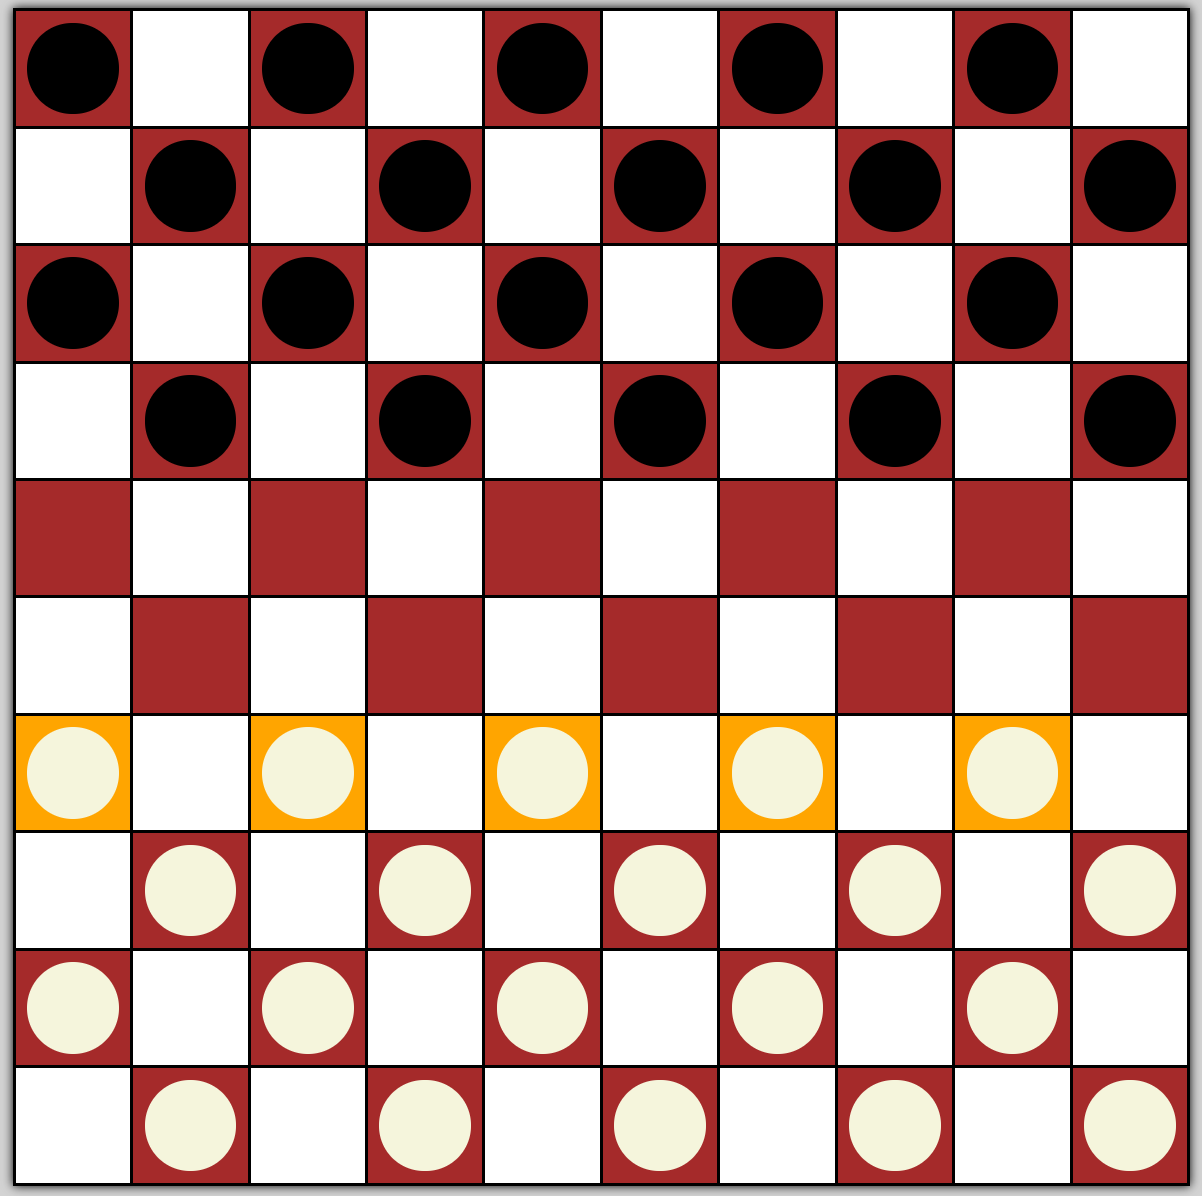
\includegraphics[width=0.5\linewidth]{pics/checkersboard.png}
	\captionof{figure}[DameSpielfeld]{ Das 10x10 Spielfeld aus der Anwendung }
	\label{fig:checkersboard}
\end{minipage}

\subsection{Minimax}
Der Minimax Algorithmus wird verwendet, um einen optimalen Spielzug in Spielen mit perfekter Information, bei zwei Spielern
zu finden. Dazu wird ein eine Baumstruktur verwendet, welche den Zustand des Spielbrettes als Knoten hat, siehe Abbildung \ref{fig:minimax}.
Alle Züge, die von einer Stellung aus möglich sind, werden in den Kindknoten des jeweiligen Knotens gespeichert.
Der Wurzelknoten beschreibt den momentanen Zustand des, Spieles bei dem der Algorithmus aufgerufen wird. Die Blattknoten am Ende des Baumes
entsprechen entweder einer Stellung in der das Spiel beendet wurde, oder der Stellung bei einer Tiefe, bei der der Algorithmus 
aufgehört hat zu suchen. Die Angabe einer Tiefe ist nötig,
da Spiele wie Schach oder Dame einen extrem großen Suchbaum zur Folge hätten und das Suchen eines Endzustandes in diesen sehr viel Zeit
beansprucht. \cite{MinimaxComparison}


Zum Beispiel kann die Abbildung \ref{fig:minimax} durch den Baum aus der Grafik \ref{fig:value}, mit einer Suchtiefe von vier, dargestellt werden.
Dabei wird jeder Terminal-Knoten, ein Knoten bei dem das Spiel vorbei ist oder die Endtiefe erreicht wurde (im Beispiel Grün makiert), 
mit einer Bewertungsfunktion bewertet:
\begin{itemize}
    \item Normale Figur: +1 für Weiß und -1 für Schwarz
    \item Dame: +3 für Weiß und -3 für Schwarz
    \item Spielende: +40 für Weiß und -40 für Schwarz
\end{itemize} 
Ein Dreieck mit der lange Seite nach unten, steht für eine Maximierung der Kindknotenwerte, das andere Dreieck für eine
Minimierung. Die Bewertungen in den Endzuständen werden nach oben durchgereicht und je nachdem ob der Elternknoten ein Maximierer oder ein
Minimierer ist bekommt er einen neuen Wert zugewiesen.
Im Beispiel kann man sehen, dass egal welche Züge gewählt werden es immer zu einem Materialverlust von Weiß kommt. Würde Weiß
die zweite Option wählen, so ist das Spiel nach dem Nächsten Zug von Schwarz schon entschieden und Weiß verliert. 


\begin{figure}[H]
\centering
\scalebox{0.7}
{%
\begin{forest}
[{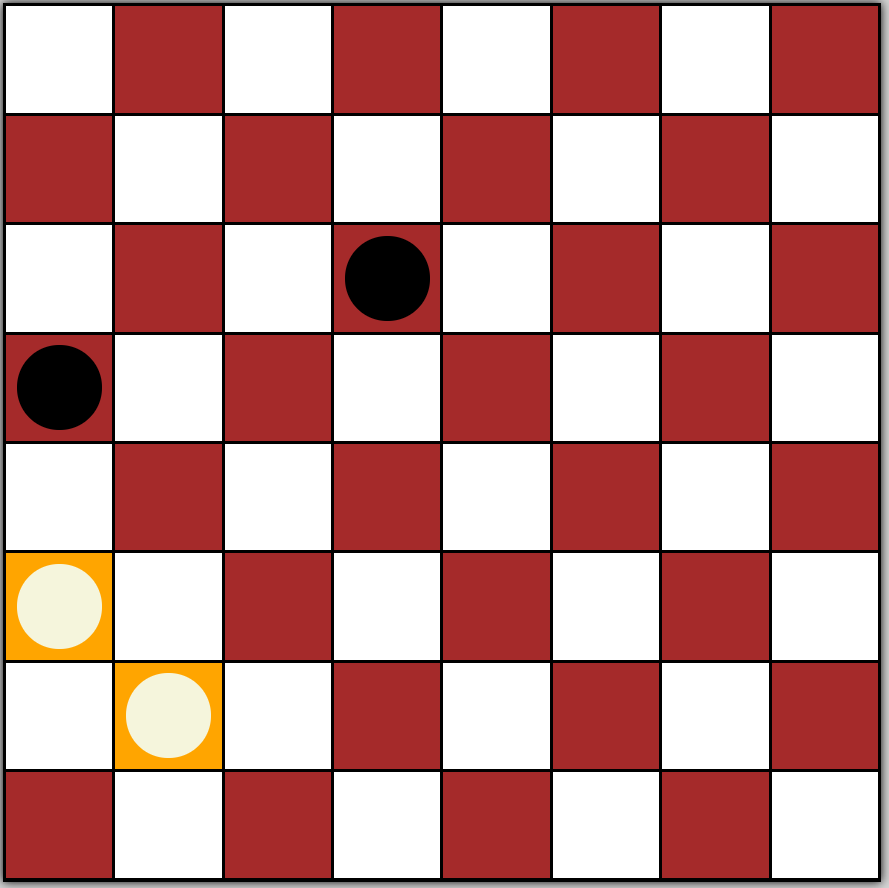
\includegraphics[scale=0.2]{pics/root.png}}
    [{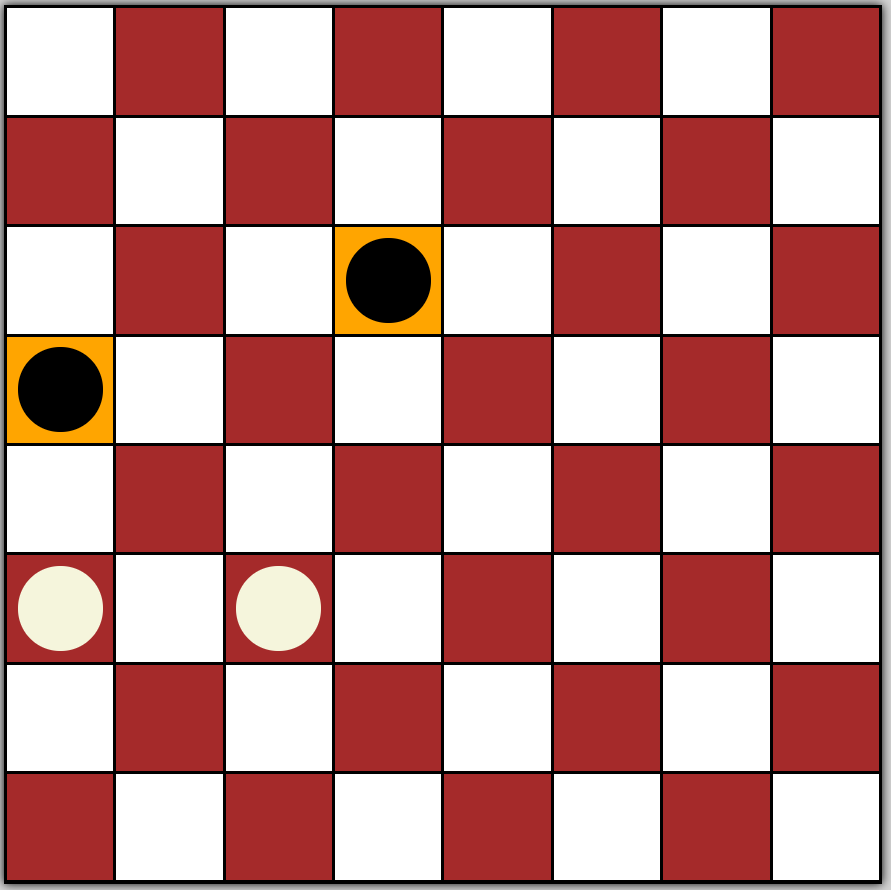
\includegraphics[scale=0.15]{pics/1goodmove.png}}
        [{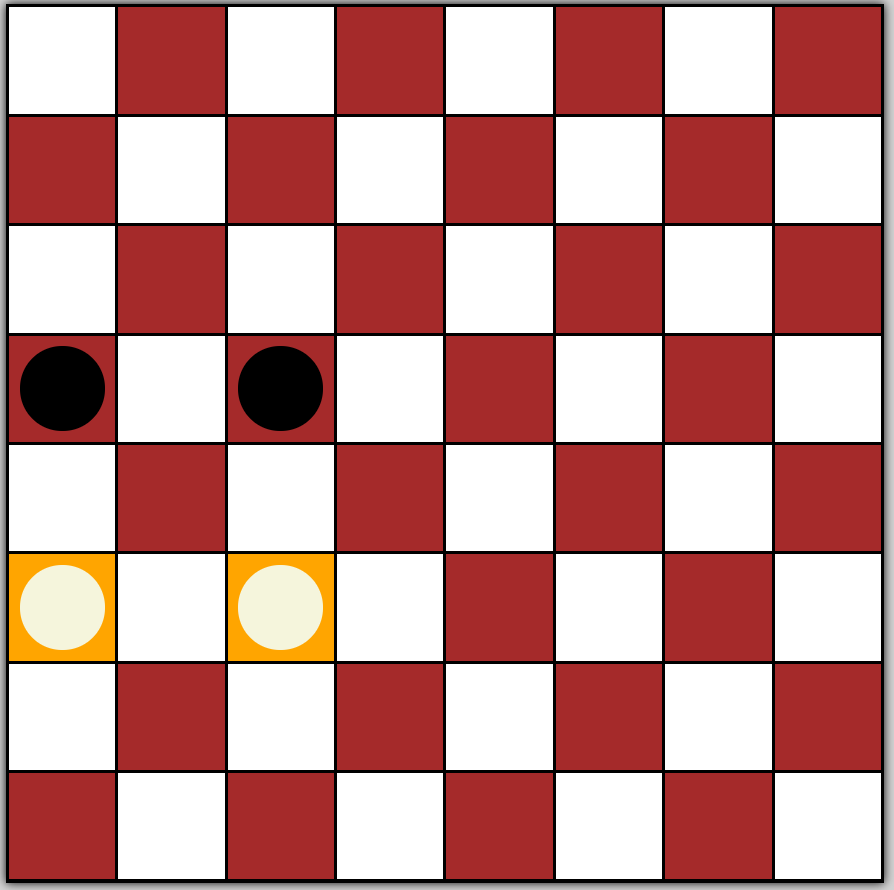
\includegraphics[scale=0.15]{pics/21goodmove.png}}
            [{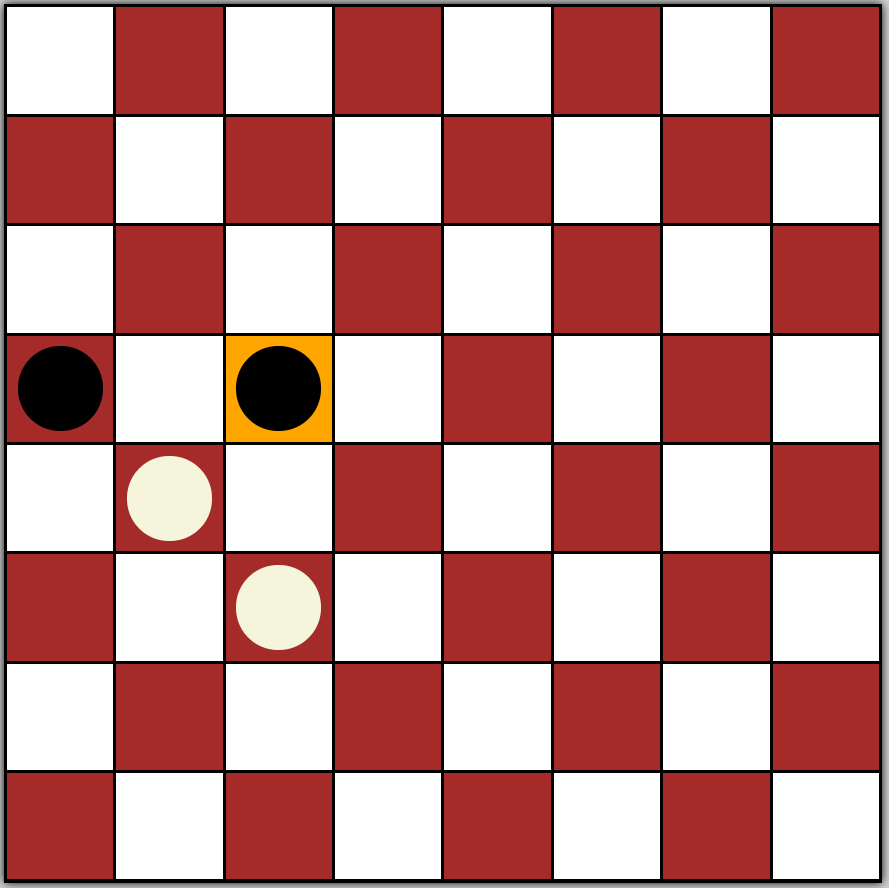
\includegraphics[scale=0.12]{pics/311goodmove.png}}
                [\vdots]
            ]
            [{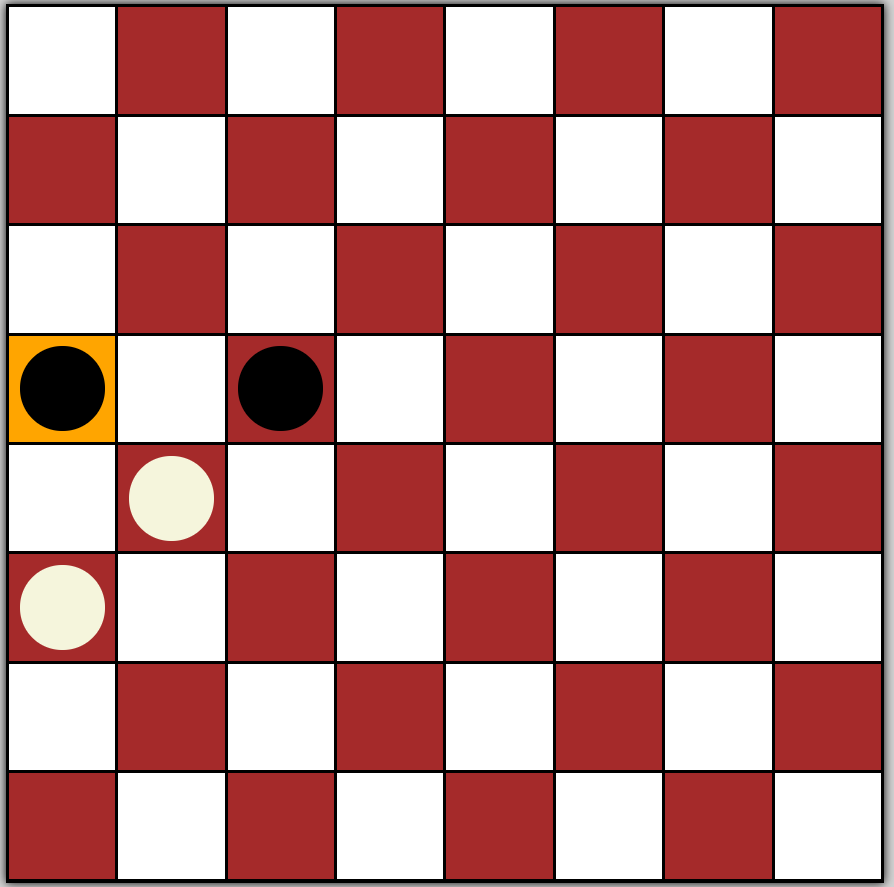
\includegraphics[scale=0.12]{pics/312goodmove.png}}
                [\vdots]
            ]
            [{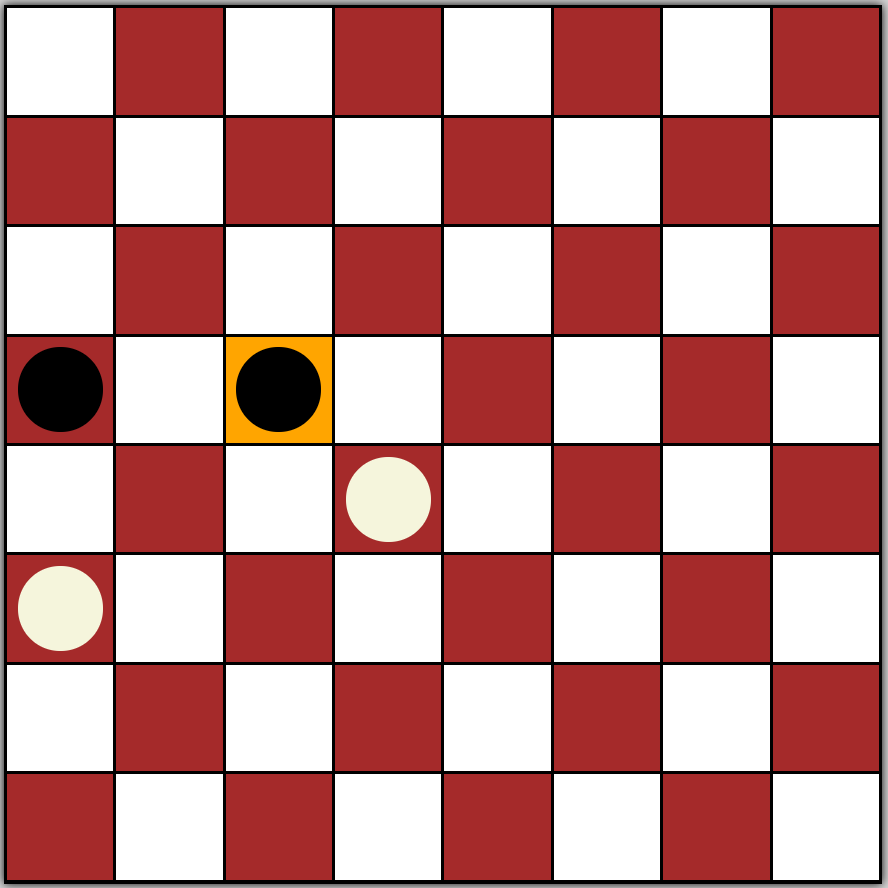
\includegraphics[scale=0.12]{pics/313goodmove.png}}
                [\vdots]
            ]
        ]
        [{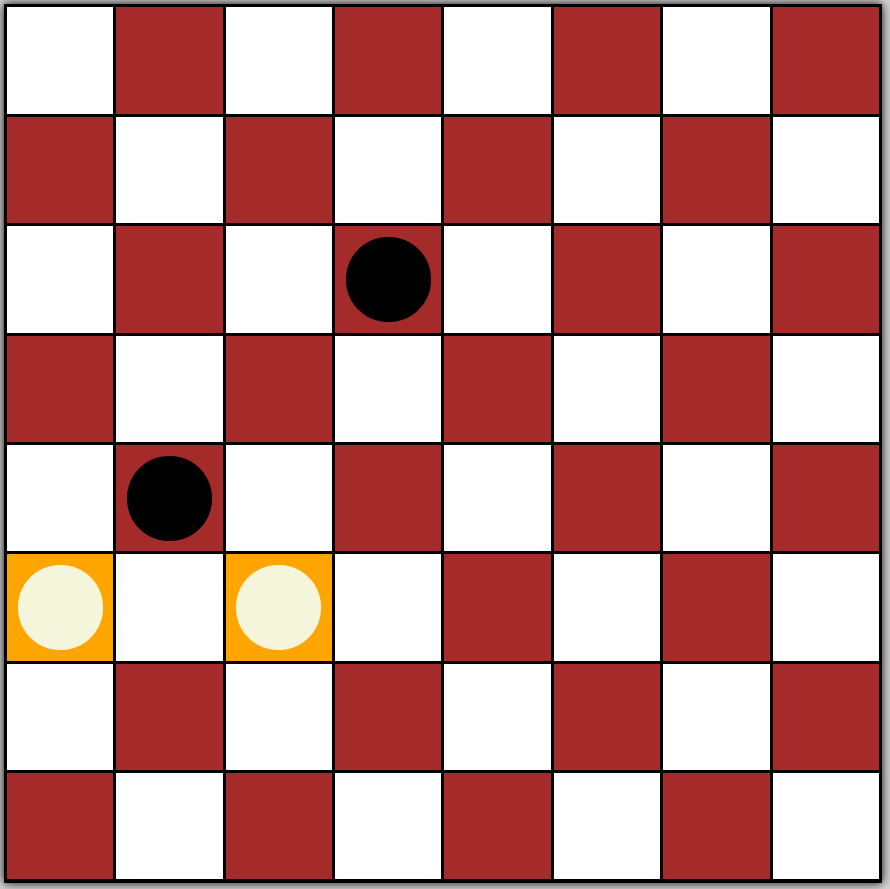
\includegraphics[scale=0.15]{pics/22badmove.png}}
            [{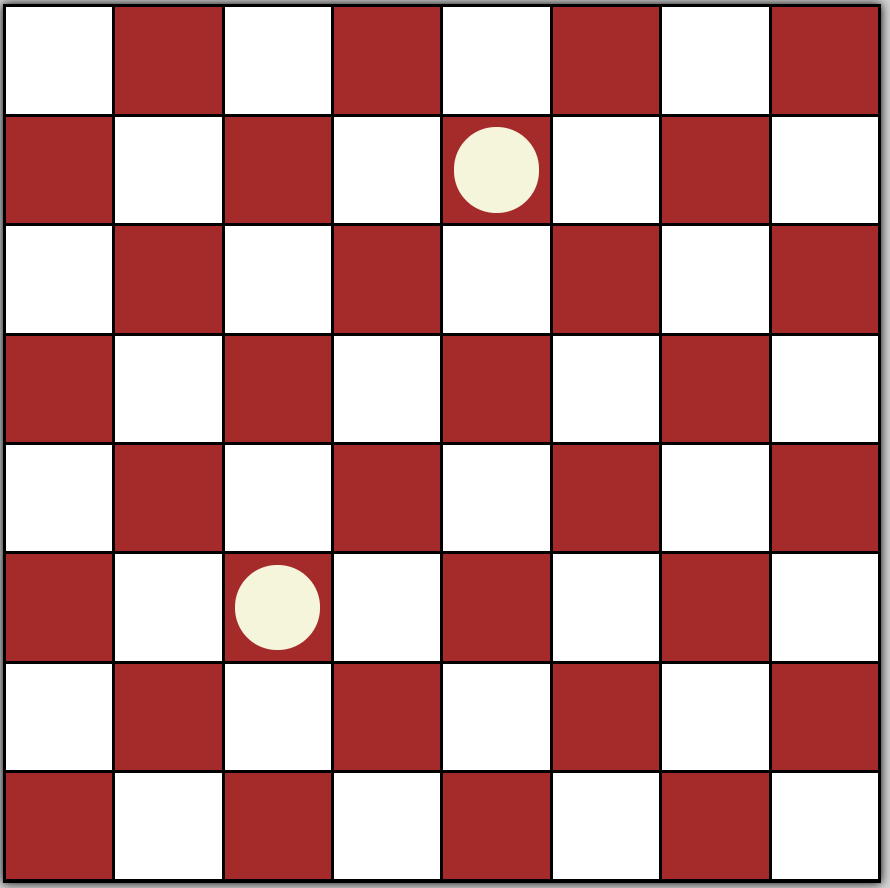
\includegraphics[scale=0.12]{pics/322badmove.png}}]
            [{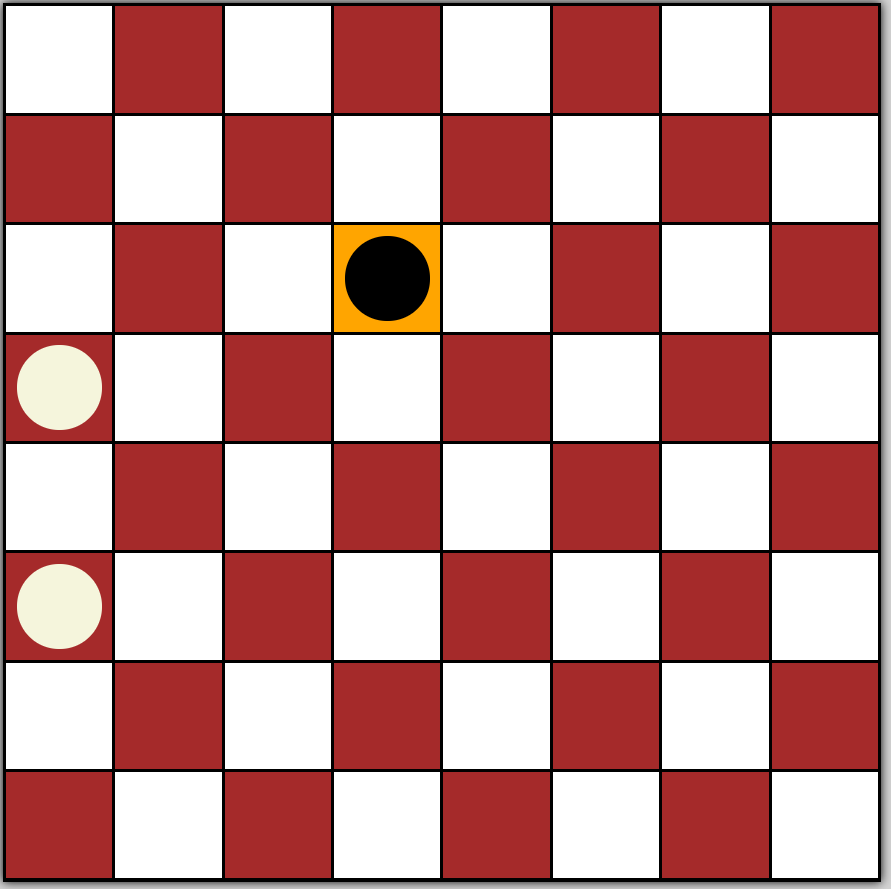
\includegraphics[scale=0.12]{pics/321badmove.png}}
                [\vdots]
            ]
        ]
    ]
    [{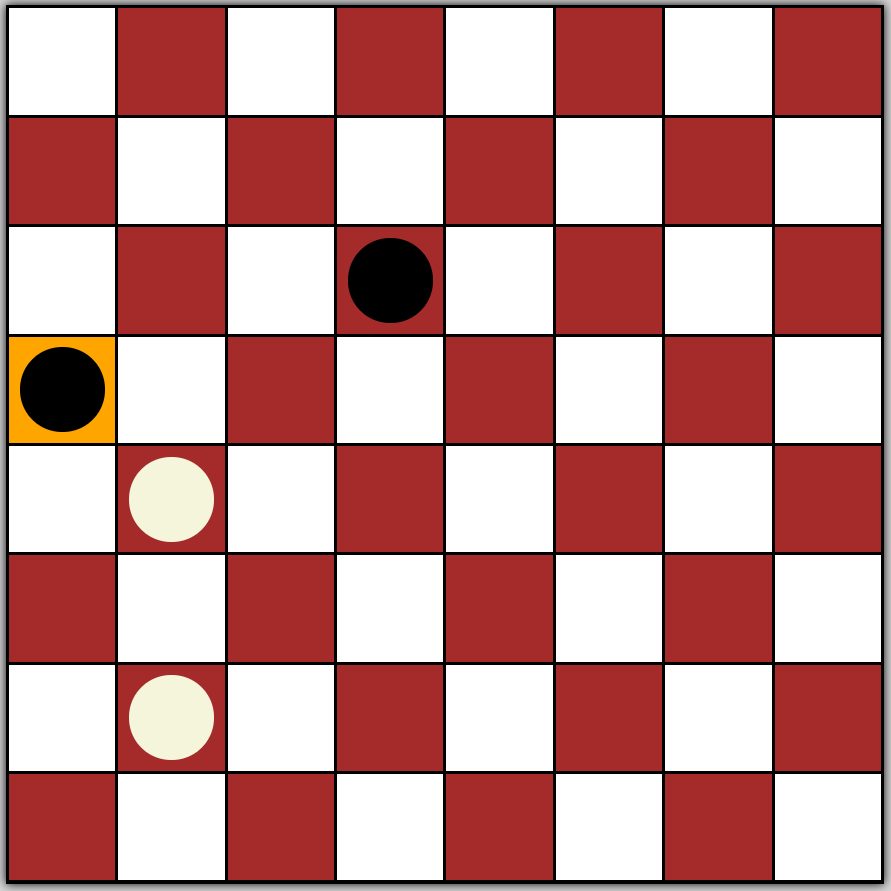
\includegraphics[scale=0.15]{pics/1badmove.png}}
        [{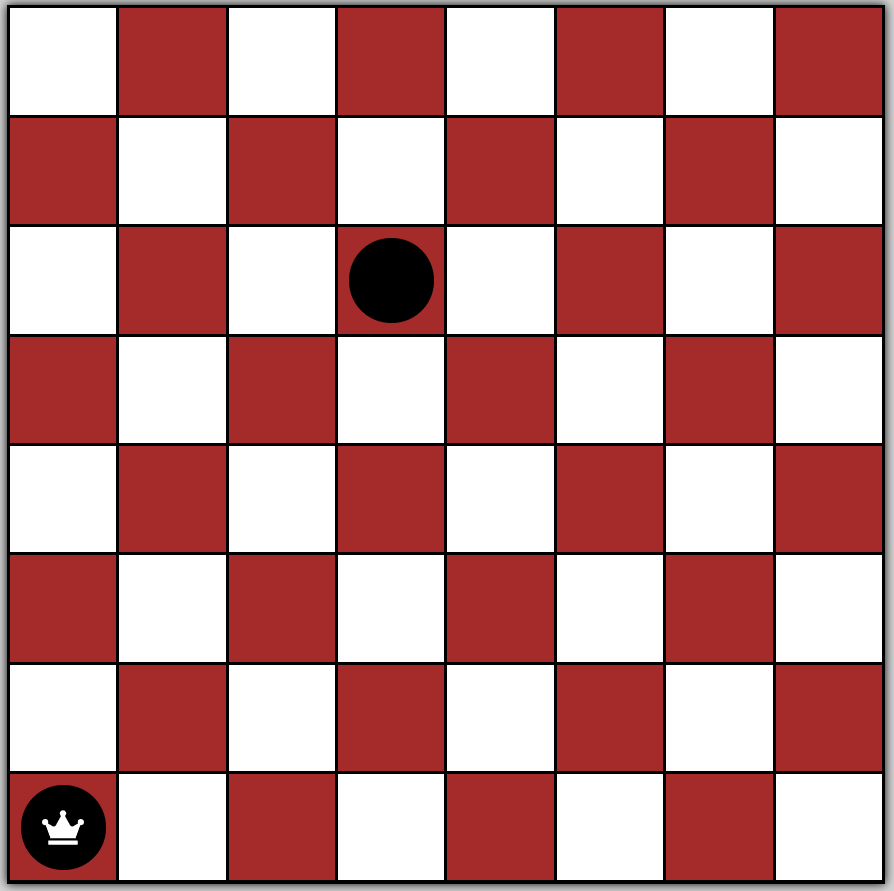
\includegraphics[scale=0.15]{pics/2winAfter1badmove.png}}]
    ]
]
\end{forest}
}
\caption{Minimax-Baum mit Spielfeldzustand als Knoten}
\label{fig:minimax}
\end{figure}

\begin{figure}[H]
\centering
{%
\begin{forest}
    [-1, upsideTria
        [-1, downsideTria
            [-1, upsideTria
                [-1, downsideTria
                    [-1, upsideTriaTerm]
                ]
                [-1, downsideTria
                    [-1, upsideTriaTerm]
                ]
                [-1, downsideTria
                    [-1, upsideTriaTerm]
                ]
            ]
            [42, upsideTria
                [42, downsideTriaTerm]
                [-1, downsideTria
                    [-1, upsideTriaTerm]
                    [-1, upsideTriaTerm]
                ]
            ]
        ] 
        [{\fontsize{9}{8}\selectfont -44}, downsideTria
            [{\fontsize{9}{8}\selectfont -44}, upsideTriaTerm]
        ] 
    ]
\end{forest}
}
\caption{Minimax-Baum mit Bewertung der Stellungen}
\label{fig:value}
\end{figure}


%\vspace{1em}
%\begin{minipage}{\linewidth}
%	\centering
%	\includegraphics[width=0.5\linewidth]{pics/minimax.png}
%	\captionof{figure}[minimax]{ Beispiel eines Minimax Suchbaumes }
%	\label{fig:minimax}
%\end{minipage}

\subsection{Iterative Deepening}
In komplexeren Spielen wie Go, Schach oder Dame ist es wegen dem Rechenaufwand sehr schwer den kompletten Baum von Minimax bis zu den
Endzuständen aufzubauen. Deswegen wird in diesen Spielen der Baum nur bis zu einer gewissen Tiefe aufgebaut. Da es aber bei einer gleichen
Tiefe für verschiedene Stellungen zu unterschiedlichen Dauern der Suche kommen kann, ist es problematisch eine fixe Suchtiefe anzugeben, 
vor allem wenn mit Zeitlimits gearbeitet wird. Iterative Deepening hilft hierbei, der Ablauf des Algorithmus ist wie folgt:
Zuerst führe Minimax für eine Tiefe von eins aus. Danach, verwerfe alle generierten Knoten des Baumes und starte erneut von Anfang, aber dieses
Mal bis zu einer Tiefe von zwei. Dieses verwerfen und neu starteten wird so oft wiederholt bis ein Zeitlimit erreicht wird, siehe Abbildung \ref{fig:IterativeDeepening}. 
Der letzte aufgebaute Baum, bevor neugestartet wird, wird zwischengespeichert und falls Minimax bis zum Ablauf des Zeitlimits nicht fertig ist,
wird die momentane Berechnung verworfen und der letzte gespeicherte Baum verwendet. Ein Nachteil dieser Methode ist, dass 
der Rechenaufwand der ersten Tiefen verschwendet wird, da diese Ergebnisse verworfen werden. Jedoch beeinflusst diese 
verschwendete Rechenzeit nicht die Asymptotische Laufzeit des Algorithmus, da die meiste Arbeit in der untersten Tiefe der 
Suche gebraucht wird. \cite{IterativeDeepening}.

\begin{figure}[H]
\centering
\begin{tabular}{*{6}{|T}}
    Tiefe 1 & Tiefe 2 & Tiefe 3 \\
    \begin{forest}
        [$\triangle$
            [$\nabla$] 
            [$\nabla$] 
        ]
    \end{forest}
    &
    \begin{forest}
        [$\triangle$
            [$\nabla$ 
                [$\triangle$]
                [$\triangle$]
            ]
            [$\nabla$ 
                [$\triangle$]
            ]
        ]
    \end{forest}
    &
    \begin{forest}
        [$\triangle$
            [$\nabla$ 
                [$\triangle$
                    [$\nabla$]
                ]
                [$\triangle$
                    [$\nabla$]
                    [$\nabla$]
                ]
            ]
            [$\nabla$ 
                [$\triangle$
                    [$\nabla$]
                    [$\nabla$]
                    [$\nabla$]
                ]
            ]
        ]
    \end{forest}
    \\
\end{tabular}
\caption{Ablauf des Iterativen Deepenings}
\label{fig:IterativeDeepening}
\end{figure}

\subsection{Alpha-Beta Pruning}
Das Alpha-Beta Pruning ist eine Optimierung zum Minimax Algorithmus. Die Idee des Algorithmus ist, 
dass manche Zweige des Suchbaums nicht untersucht werden müssen, da für den anderen Spieler diese
Züge nicht in Frage kommen. Hierbei ist $\alpha$ der Wert für den Spieler, für den die niedrigen Werte 
besser sind und $\beta$ für den anderen Spieler. Für jeden Knoten, je nachdem, ob er ein maximierender
oder ein minimierender Knoten ist, wird überprüft, ob ein Kind-Knoten, welcher einen neuen Wert
erhalten hat, nicht mehr vom Knoten beachtet werden muss. Der Vorteil des Alpha-Beta Prunings zu Minimax ist, 
dass der verbrauchte Speicher weniger wird, da vom Baum Zweige nicht beachtet werden müssen.
Was wiederum zur Folge hat das die Ausführungszeit des Algorithmus schneller ist und gleichzeitig auch dasselbe 
Ergbnis wie Minimax zur Folge hat.
\cite{AlphaBeta}

Wenn man Abbildung \ref{fig:minimax} und \ref{fig:value} als Beispiel nimmt und den Alpha-Beta Pruning Algorithmus anwendet,
so kann der Zweig mit dem Wert 42 ignoriert werden, siehe Abbildung \ref{fig:AlphaBeta}. Der gelbe Knoten bekommt eine -1 
durch seinen linken Zweig vorübergehend zugewiesen. Da der Knoten des Rechten Zweiges ein Maximierer ist, also immer den Wert des
Kindknotens mit dem höchsten Wert nimmt, und dieser bereits einen Knoten mit dem Wert 42 gefunden hat, wird sein Wert 
definitiv mindestens 42 sein. Der restliche Rechte Zweig des gelben Knotens kann nun ignoriert werden, da der linke Zweig mit
-1 definitiv kleiner sein wird.

\begin{figure}[H]
\centering
{%
\begin{forest}
    [-1 , upsideTria
        [-1, downsideTriaYellow
            [-1, upsideTria
                [-1, downsideTria
                    [-1, upsideTriaTerm]
                ]
                [-1, downsideTria
                    [-1, upsideTriaTerm]
                ]
                [-1, downsideTria
                    [-1, upsideTriaTerm]
                ]
            ]
            [42, upsideTria, edge={myedge}
                [42, downsideTriaTerm]
                [?, downsideTria]
            ]
        ] 
        [{\fontsize{9}{8}\selectfont -44}, downsideTria
            [{\fontsize{9}{8}\selectfont -44}, upsideTriaTerm]
        ] 
    ]
\end{forest}
}
\caption{Gewinn durch Alpha-Beta Pruning}
\label{fig:AlphaBeta}
\end{figure}

\subsection{Zugsortierung}
Zugsortierung ist ein Zusatz zur Alpha-Beta Suche.
Da Alpha-Beta Pruning abhängig von der Reihenfolge, in der die Zustände untersucht werden ist, ist es sinnvoll
die Nachfolger zu wählen, die die besten Werte erbringen. Den besten Nachfolger findet man, in dem man eine
weitere Bewertungsfunktion einbaut, welche nicht so genau wie die Bewertungsfunktion an den Terminalknoten sein muss. 
Wenn ein Knoten also alle möglichen Nachfolgezüge als Kinder bekommt, werden auf diese die vereinfachte Bewertungsfunktion
angewandt und, je nach Ergebnis der Funktion werden die Nachfolger sortiert. Dadruch, dass der beste Zug nun
sehr weit am Anfang steht, ist es sehr wahrscheinlich das die anderen Züge durch Alpha-Beta Pruning ignoriert werden.
\cite{KuenstlicheIntelligenzNorvig}

Auf der Linken Seite der Abbildung \ref{fig:Sorting} kann man erkennen, dass Alpha-Beta Pruning keinen Effekt 
auf die beiden gelben Knoten hätte. Ändert man jedoch die Reihenfolge der Knoten, so kann der Knoten mit dem Wert 42
ignoriert werden. Bei der Bewertungsfunktion könnte man die bedrohte Figuren als Faktor haben, um auf dieses Ergbnis zu kommen.


\begin{figure}[H]
\centering
{%
\begin{forest}
    [-1, upsideTria
        [-1, downsideTria
            [42, upsideTriaYellow
                [42, downsideTriaTerm]
                [-1, downsideTria
                    [-1, upsideTriaTerm]
                    [-1, upsideTriaTerm]
                ]
            ]
            [-1, upsideTriaYellow
                [-1, downsideTria
                    [-1, upsideTriaTerm]
                ]
                [-1, downsideTria
                    [-1, upsideTriaTerm]
                ]
                [-1, downsideTria
                    [-1, upsideTriaTerm]
                ]
            ]
        ] 
        [{\fontsize{9}{8}\selectfont -44}, downsideTria
            [{\fontsize{9}{8}\selectfont -44}, upsideTriaTerm]
        ] 
    ]
\end{forest}
\raisebox{1\height}{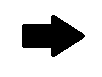
\includegraphics{pics/ArrowRight.png}}
\begin{forest}
    [-1 , upsideTria
        [-1, downsideTria
            [-1, upsideTriaYellow
                [-1, downsideTria
                    [-1, upsideTriaTerm]
                ]
                [-1, downsideTria
                    [-1, upsideTriaTerm]
                ]
                [-1, downsideTria
                    [-1, upsideTriaTerm]
                ]
            ]
            [42, upsideTriaYellow, edge={myedge}
                [42, downsideTriaTerm]
                [?, downsideTria]
            ]
        ] 
        [{\fontsize{9}{8}\selectfont -44}, downsideTria
            [{\fontsize{9}{8}\selectfont -44}, upsideTriaTerm]
        ] 
    ]
\end{forest}
}
\caption{Beispiel einer Zugsortierung}
\label{fig:Sorting}
\end{figure}

\subsection{Monte Carlo Tree Search (MCTS)}
Der Monte Carlo Tree Search Algorithmus, ist ein heuristischer Algorithmus, bei welchem von einem
Zustand eines Spieles zufällig endlich viele Simulationen durchgeführt werden. Die Simulation endet, wenn
ein Ergebnis des simulierten Spieles feststeht. Das Wiederholen der Simulationen aus verschiedenen Knoten
hat zur Folge, dass das Ergebnis immer genauer wird. Am Ende wird der Knoten gewählt, bei dem die 
Simulationen die besten Ergebnisse für den momentanen Spieler gezeigt haben. Ein Vorteil des 
MCTS-Algorithmus gegenüber Minimax ist, dass erst am Ende eines Durchlaufs eine Bewertungsfunktion
benötigt wird. Allgemin besteht der Algorithmus aus vier Schritten:
\begin{itemize}
    \item \textit{Selektion}: Versucht wird, einen Zustand zu finden der noch erweiterbar ist, also
        einen Zustand zu finden, der kein Endzustand ist und noch nicht besuchte Züge hat.
    \item \textit{Expansion}: Der Spielbaum wird zufällig um einen noch nicht besuchten Zug erweitert.
    \item \textit{Simulation}: Von dem gewählten Knoten aus wird nun ein Spiel zufällig bis zum Ende 
        simuliert. 
    \item \textit{Backpropagation}: Das Ergebnis der Simulation wird den vorhergehenden Knoten mitgeteilt
        und diese werden mit diesem aktualisiert.
\end{itemize}
Da man im Normalfall nicht beliebig viel Zeit hat alle Möglichkeiten zu simulieren, versucht man die limitierte Zeit
so gut wie möglich zu nutzen und die richten Knoten zum Expandieren zu wählen. Dazu wird der \textit{upper confidence bound for trees} (UCT) verwendet.
Die UCT Formel lautet:
\begin{align}
	w + c \sqrt{\frac{\log{N}}{n}}
\end{align}
Wobei $w$ die prozentuale Anzahl an Gewinnen des Knotens, $N$ die Anzahl der gesamten Expansionen und $n$ die Expansionen nur an dem 
betrachteten Knoten sind. Die Aufgabe der UCT Formel ist das Erreichen von zwei im Konflikt stehenden Zielen. Das erste Ziel ist es die Knoten die bisher die 
höchsten Chancen auf den Gewinn haben tiefer zu simulieren, um eine bessere Genauigkeit des besten Zuges zu haben.
Das zweite Ziel ist Knoten, die noch nicht sehr oft besucht worden sind genauer zu untersuchen, da diese vielversprechender sein könnten als gedacht.
Für die Balancierung der beiden Ziele gibt es den Parameter $c$ \cite{DeepLearingGo}.

Als Beispiel wird die zuvor verwendete Stellung aus \ref{fig:minimax} benutzt, aus welcher der MCTS-Baum in Abbildung \ref{fig:MCTSTree} entsteht.
"`B"' steht für die Siege aus Schwarzer und "`W"' für Siege aus Weißen Sicht, nach der Beendigung von 33 Simulationen.  
Weiß entscheidet sich in diesem Baum für den gelben Knoten, da dieser bei Betrachtung der Gewichtung von Siege eine höhere
Gewinnchance für ihn hat.

\begin{figure}[H]
\centering
{%
\begin{forest}
    for tree={%
        edge={->},
    }
    [B:27 W:6, circle, draw
        [B:19 W:6, circle, fill=yellow, draw
            [B:12 W:1, circle, draw
                [B:4 W:1, circle, draw
                    [B:4 W:1, circle, draw [{\vdots}]]
                ]
                [B:3 W:0, circle, draw
                    [B:3 W:0, circle, draw [{\vdots}]]
                ]
                [B:5 W:0, circle, draw
                    [B:5 W:0, circle, draw [{\vdots}]]
                ]
            ]
            [B:7 W:5, circle, draw
                [B:0 W:4, circle, draw]
                [B:7 W:1, circle, draw
                    [B:3 W:1, circle, draw [{\vdots}]]
                    [B:4 W:0, circle, draw [{\vdots}]]
                ]
            ]
        ] 
        [B:8 W:0, circle, draw
            [B:8 W:0, circle, draw]
        ] 
    ]
\end{forest}
}
\caption{Minimax-Baum mit Bewertung der Stellungen}
\label{fig:MCTSTree}
\end{figure}

%\section{Anforderungsanalyse}
%In diesem Kapitel wird zuerst ein beispielhaftes Szenario gezeigt, bei welchem die Software eingesetzt werden soll.
%Anschließend werden anhand dieser Szenarios Anforderungen definiert, die von der Software erfüllt werden müssen.
%\subsection{Anwendungsszenario}
%Will ein Benutzer gegen den KI Client spielen, kann er über das Menü auf dem Touch Monitor den KI Algorithmus auswählen und diesen herausfordern.
%Dazu kann er, falls er mit seinem Smarthphone spielen will einen QR-Code auf dem Monitor aufrufen, diesen einscannen und dann das Spiel beginnen.
%Andernfalls kann der Benutzer auch direkt am Monitor das Spiel starten und auf diesen mittels Touch Züge ausführen.
%Die KI Algorithmen welche auf dem KI Client implementiert sind haben eine ELO Zahl hinterlegt, welche Auskunft über die Spielstärke gibt.
%Fühlt sich der Benutzer also über oder unterfordert, kann er den geeigneten Gegner auswählen. Gibt es mehrere Benutzer welche 
%gegen einander spielen wollen, haben diese die Möglichkeit entweder abwechselnd auf dem Monitor, oder beide mittels QR-Code über ihr Smartphone ein Spiel zu starten.
%Will ein Benutzer zwei KI's beim Spielen beobachten, so kann er diese am Monitor auswählen und diese gegeneinander Antreten lassen.
%\subsection{Anforderungen an die Software}
%Aus dem oben beschriebenen Anwendungsszenario lassen sich konkrete Anforderungen ableiten, die für die Software von Relevanz sind.
%Hierbei wird zwischen funktionalen und nicht funktionalen Anforderungen unterschieden \cite{RequirementEngenieering}.
%\subsubsection{Funktionale Anforderungen}
%\begin{itemize}
%    \item \textbf{/F10/} \textit{Menü zum Auswählen des Spieles:} Die Grafische Oberfläche soll dem Benutzer die Möglichkeit geben, das ein Spiel auszuwählen.
%        Dazu soll es ein Menü geben welches die möglichen Spiele, wie z.B. Reversi oder Dame zur Auswahl stellt.
%    \item \textbf{/F11/} \textit{Auswählbares Menü für verschiedene KI Algorithmen:} Die Applikation muss ein leicht bedienbares Grafisches Interface bieten,
%        bei welchem verschiedene künstliche Intelligenz Algorithmen ausgewählt und herausgefordert und werden können.
%    \item \textbf{/F12/} \textit{QR-Code fürs verbinden mit dem Smartphone:} Um einen unkomplizierten Verbindungsaufbau vom Raspberry mit dem Smarthphone zu 
%        gewährleisten, soll es eine Menü-Option geben, bei der ein QR-Code angezeigt wird. Nach dem Scannen des QR-Codes soll eine Verbindung
%        aufgebaut werden, welche bis zum Beenden bestehen bleibt.
%    \item \textbf{/F13/} \textit{Varaible Zeiteinstellung im Menü:} Dem Benutzer soll es möglich sein über das Menü eine Zeit einstellen zu können, 
%        welche jeder Spieler im Spiel zur Verfügung für seine Züge hat. Als Spieler können entweder Benutzer oder KI Clients agieren.
%    \item \textbf{/F20/} \textit{Benutzer soll Züge ausführen können:} Der Benutzer soll in der Lage sein, Züge gegen die KI spielen zu können. Dazu soll er entweder
%        direkt über den Touch-Monitor oder über das Smartphone eine Eingabemöglichkeit haben. Diese soll den Momentanzustand des Spielbrettes zeigen,
%        wodurch der Benutzer eine Entscheidung für seinen nächsten Zug treffen und diese über eine Touch-Berührung ausführen kann.
%    \item \textbf{/F21/} \textit{Benutzer sollen gegen andere Benutzer spielen können:} Für mehrere Benutzer soll es möglich sein, gegeneinander spielen zu können. Dazu sollen sie 
%        entweder den Touch-Monitor verwenden, indem sie abwechselnd Züge ausführen, oder beide jeweils ein Smarthphone.
%    \item \textbf{/F22/} \textit{Der Benutzer kann KI's gegeneinander spielen lassen:} Der Benutzer soll in der Lage sein zwei KI-Algorithemen auszuwählen
%        und diese gegeneinander spielen zu lassen. Damit man dieses Spiel sehe kann, sollen alle Züge die 
%        von beiden getätigt werden auf dem Spielbrett des Touch-Monitors angezeigt werden.
%    \item \textbf{/F30/} \textit{Eine ELO Zahl soll die Spielstärke der Algorithmen angeben:} Damit der Benutzer eine für sich angemessene Herausforderung findet,
%        sollen schwächere und stärkere KI-Algorithmen in der GUI gekennzeichnet werden. Um eine genaue Kennzahl für die Stärke zu erhalten, werden die ELO Zahlen durch
%        Simulationen berechnet. Diese Simulationen sind Spiele der Algorithmen untereinander.
%   
%\end{itemize}
%\subsubsection{Nichtfunktionale Anforderungen}
%\begin{itemize}
%    \item \textbf{/Q10/} \textit{Robustheit der Smarthphone Verbindung:} Nach der Verbindung mit dem Smarthphone (mittels QR-Code /F12/) muss sichergestellt sein, dass die Verbindung nicht ohne
%        Grund abbricht, sondern erst, wenn z.B. die Distanz zwischen Smartphone und Pi zu groß ist. Des weitern soll nach einem Verbindungsabbruch, 
%        das Spiel nicht abgebrochen werden, sondern es soll eine Möglichkeit zum Wiederverbinden bestehen.
%    \item \textbf{/Q20/} \textit{ELO Zahlen sollen Stärke wiederspiegeln:} Die durch die Simulationen errechnete ELO Zahl von /F30/ soll auch in etwa dem Stärkegrad der Algorithmen entsprechen.
%        Hat ein Algorithmus die sehr viel mehr ELO muss er auch dementsprechend stärker sein.
%    \item \textbf{/Q30/} \textit{Zeiteinstellung soll von der KI Berücksichtigt werden:} Die Zeiteinstellung von /F13/ soll vom KI Client als Berechnungsdauer genutzt werden.
%        Dieser soll dabei seine Rechenzeit so gut wie möglich an die Zeiteinstellung anpassen.
%    \item \textbf{/Q40/} \textit{Reaktionszeit des Touch-Interfaces:} Das Berühren des Touch-Monitors soll zur sofortigen Ausführung des Befehls der Software führen.
%    \item \textbf{/Q50/} \textit{Mobile Responsiveness:} Das Spielfeld soll auf egal welchem verbundenen Smarthphone gleich skaliert aussehen. 
%        Das Verwenden von Tablets, oder das Drehen des Gerätes soll keinen Einfluss auf die Darstellung des Spielbrettes haben.
%\end{itemize}
%\subsubsection{Zusammenfassung der Anforderungen}
%Die Identifizierten Funktionalen und Nichtfunktionalen Anforderungen werden in der Tabelle \ref{tab:Anforderungen} zusammengefasst. 
%Die Kürzel sind für die folgenden Kapietel von Relevanz da sie in diesen Referenziert werden.
%\vspace{1em}
%\begin{table}[!h]
%	\centering
%	\begin{tabular}{|l|l|l|}
%		\hline
%		\textbf{ID} & \textbf{Funktionale Anforderung}\\
%		\hline
%		/F10/ & Menü zum Auswählen des Spieles \\
%		\hline
%		/F11/ & Auswählbares Menü für verschiedene KI Algorithmen \\
%		\hline
%        /F12/ & QR-Code fürs verbinden mit dem Smartphone \\
%		\hline
%		/F13/ & Varaible Zeiteinstellung im Menü \\
%        \hline
%		/F20/ & Benutzer soll Züge ausführen können \\
%        \hline
%		/F21/ & Benutzer sollen gegen andere Benutzer spielen können \\
%        \hline
%		/F22/ & Der Benutzer kann KI's gegeneinander spielen lassen \\
%        \hline
%		/F30/ & Eine ELO Zahl soll die Spielstärke der Algorithmen angeben \\
%	
%		\hline
%		\textbf{ID} & \textbf{Nichtfunktionale Anforderung}\\
%		\hline
%		/Q10/ & Robustheit der Smarthphone Verbindung \\
%        \hline
%		/Q20/ & ELO Zahlen sollen Stärke wiederspiegeln \\
%        \hline
%		/Q30/ & Zeiteinstellung soll von der KI Berücksichtigt werden \\
%        \hline
%		/Q40/ & Reaktionszeit des Touch-Interfaces \\
%        \hline
%		/Q50/ & Mobile Responsiveness \\
%		\hline
%	\end{tabular}
%	\caption{Anforderungstabelle}
%	\label{tab:Anforderungen}
%\end{table}

\pagebreak
% ----------------------------------------------------------------------------------
% Kapitel: ???
% ----------------------------------------------------------------------------------

\section{Architektur der Software}
Dieses Kapitel setzt sich mit der Softwarearchitktur auseinander. 
%Die Architektur ist nach dem Model der Client-Server-Architektur entworfen. 
%Die Client-Server-Architektur trennt die Software in drei
%Teile, zwei Clients und einen Server: \\
%Der Gameserver, an den neue Züge geschickt werden und welcher dan Momentanzustand des Spielbrettes hält, dient als Server.
%Die ReversiXT GUI, über welche der User Spiele starten und KI's auswählen kann und dem KI Client, welcher eine künstliche Intelligenz für Dame ist, 
%sind die beiden Clients die sich mit dem Server verbinden.
\subsection{Überblick}
Um für eine bessere Modularität und Erweiterbarkeit zu sorgen, ist die Software auf drei Teile aufgeteilt.
Der Gameserver hält die Spielelogik und den Zustand des Spieles.  Über die ReversiXT Graphische Oberfläche kann man über den Gameserver 
gegen die Dame KI des KI Clients spielen. Der KI Client ist eine Dame künstliche Intelligenz, welche sich mit dem Gameserver verbindet
und die berechneten Züge an diesen sendet. 



\subsection{Kommunikation der Komponenten}
\label{chap:Ablauf}
Ein Spiel kann nur über die GUI der Applikation gestartet werden, dabei entstehen verschiedene Szenarien, abhängig davon
was der User vor dem Spiel einstellt:
\begin{itemize}
    \item Benutzer gegen Benutzer
    \item Benutzer gegen KI
    \item KI gegen KI
\end{itemize}
Egal welche Option gewählt wird, der Gameserver wird immer gestartet, da dieser die Züge überprüft und Sieg oder Niederlage auswertet.
Bei Benutzer gegen Benutzer wird die KI Komponente der Software nicht gestartet, es Kommuniziert die GUI-Komponente direkt mit Gameserver.
Wird Benutzer gegen KI gewählt, wird eine KI Komponente gestartet. Der Gameserver verbindet sich dann mit dieser und der GUI und verteilt
abwechselnd Zugaufforderungen an beide. Wird sich für zwei KI Clients die gegeneinander spielen entschieden, so werden auch zwei gestartet.
Die Kommunikation findet nur mehr von Gameserver mit den beiden KI-Clients statt, jedoch hat die GUI-Komponente eine Man-in-the-Middle-Funktion
wodurch sie die Kommunikation abhört und die gespielten Züge darstellen kann.

\subsubsection{Kommunikations Ablauf Benutzer gegen Benutzer}

\vspace{1em}
\begin{minipage}{\linewidth}
	\centering
	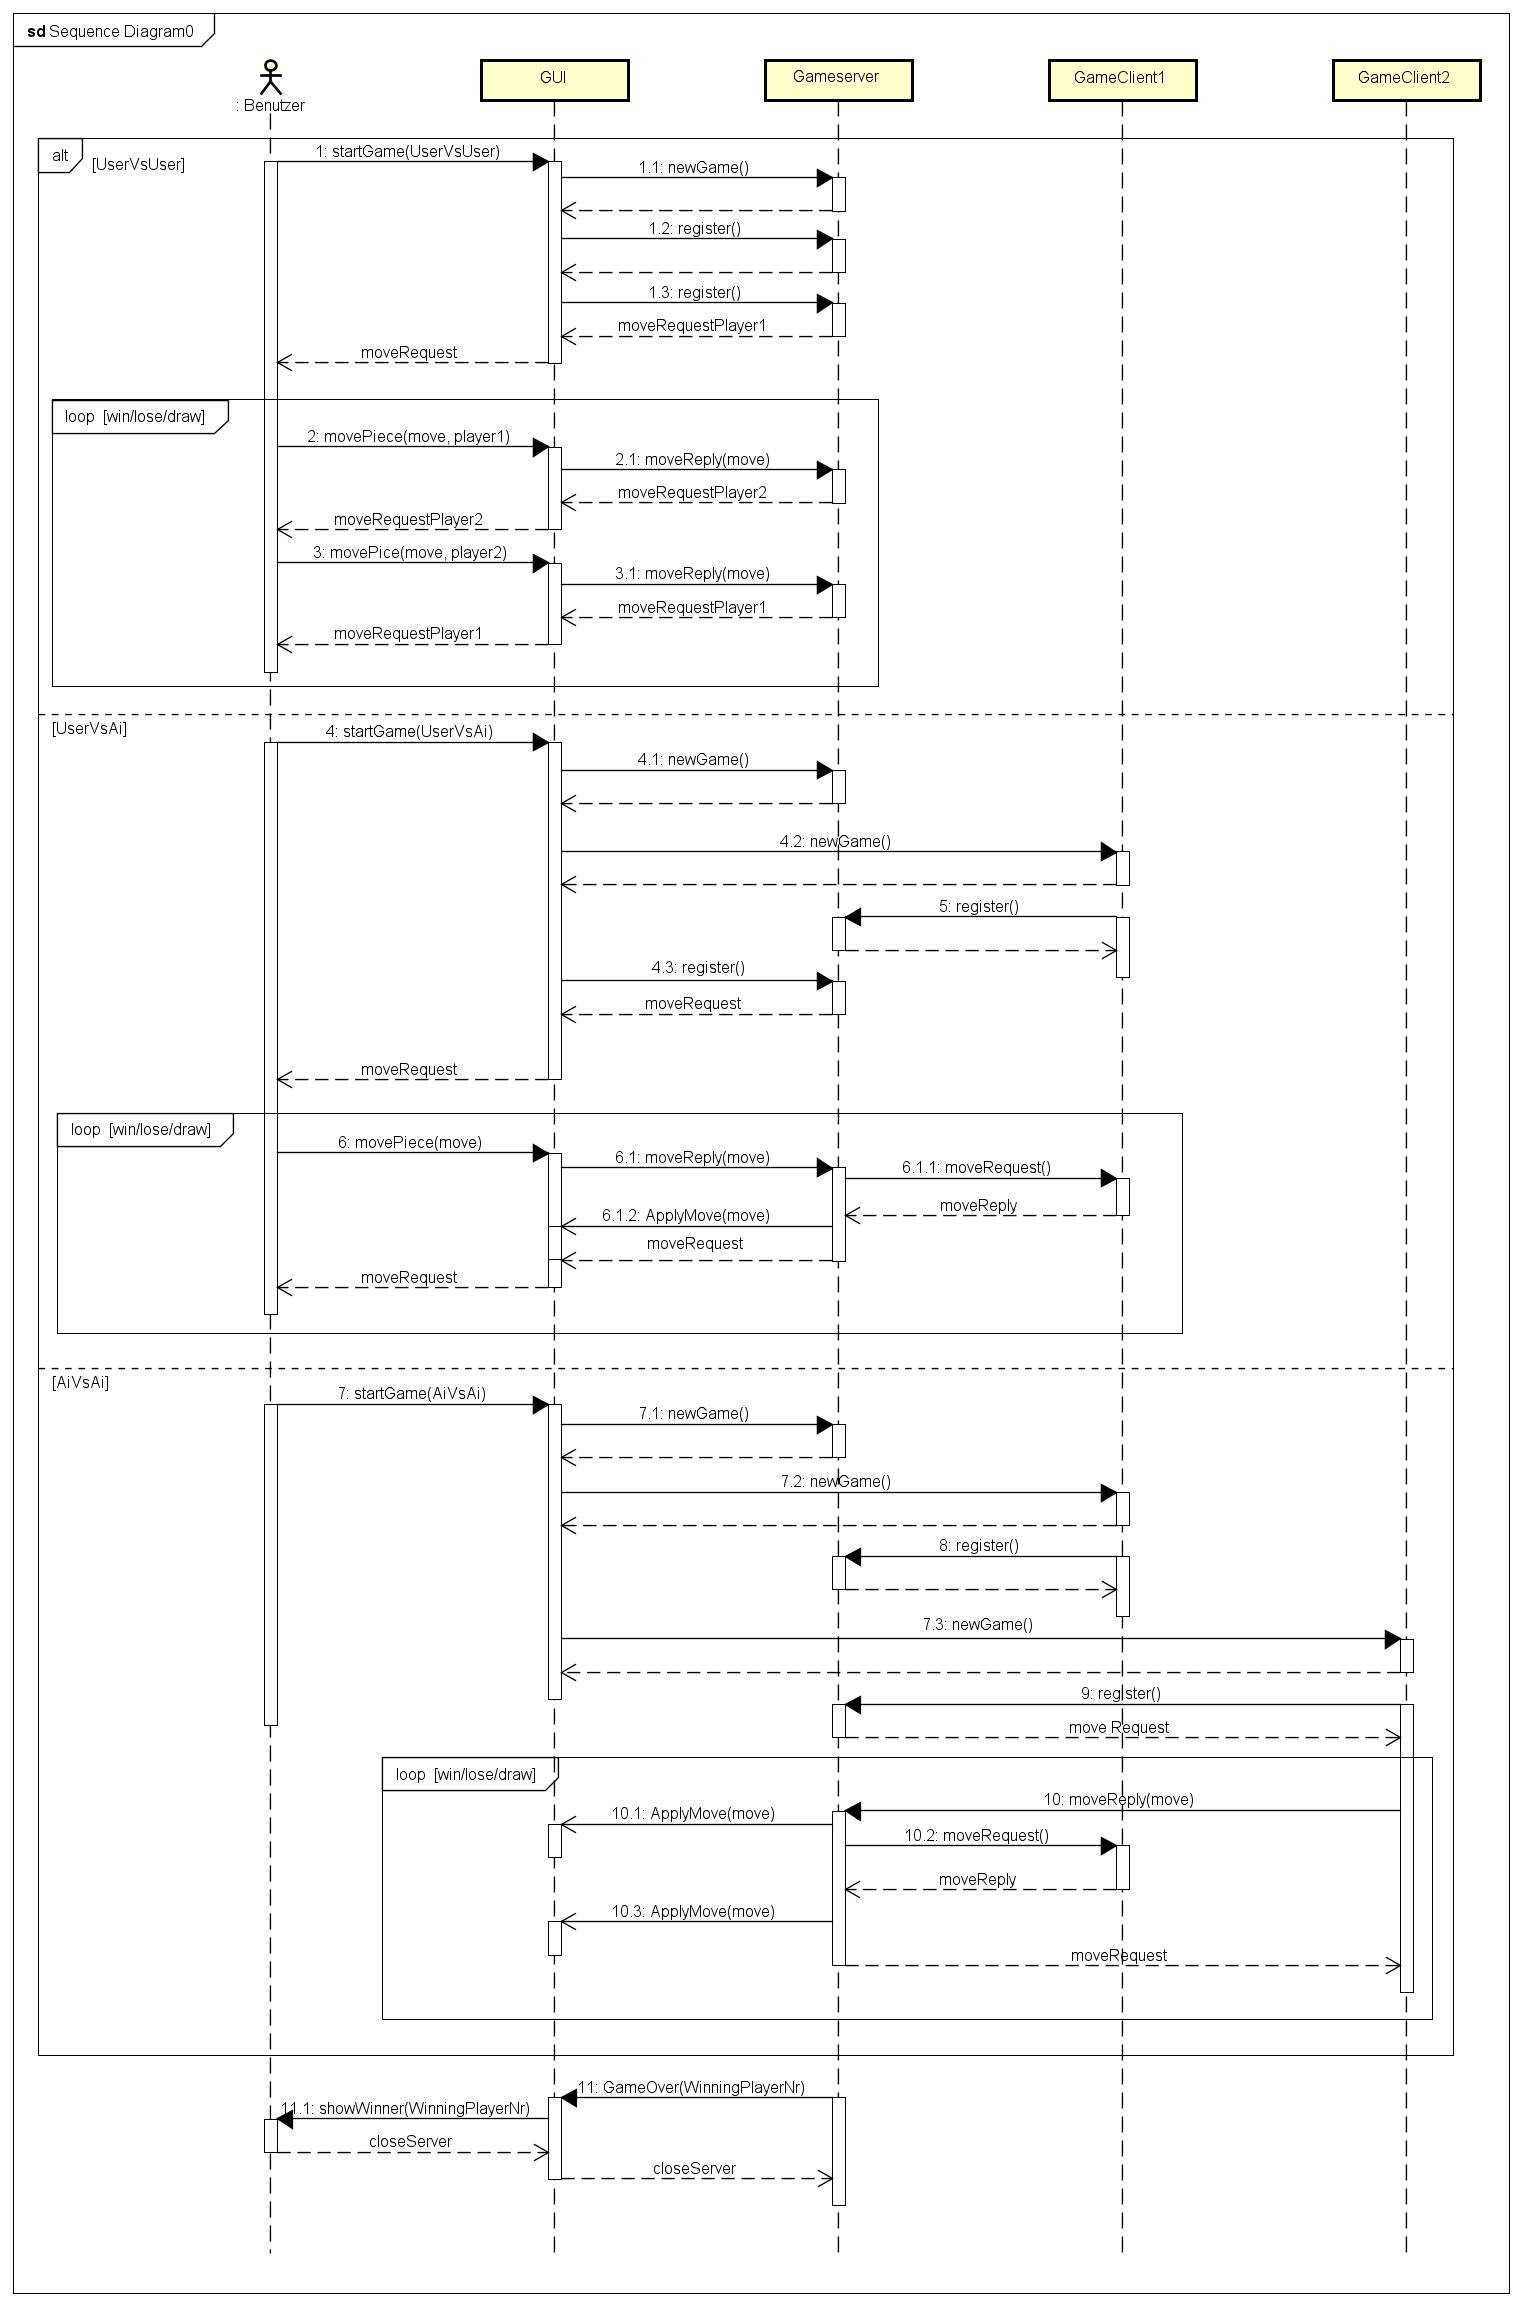
\includegraphics[width=0.83\linewidth]{pics/KommunikationSequenceDiagram.png}
	\captionof{figure}[SequenceDiagram]{ Das UML Sequenzdiagramm der Kommunikation}
	\label{fig:KommunicationSequenceDiagram}
\end{minipage}



\subsubsection{Kommunikationsprotokoll}
Im Abschnitt \ref{chap:Ablauf} wird eine Kommunikation zwischen dem Gameserver und seinen Clients beschrieben, bei welcher der 
Server nur Anfragen eines festgelegten Protokolles Akzeptiert. Das Protokoll für den Server orientiert sich stark nach dem Protokoll
des Reversi-Gameservers. 
%Nachdem ein Spiel gestartet wurde, sendet der Gameserver den Initialzustand des Spielbrettes an die Clients und
%eine Zugaufforderung an den Spieler der den ersten Zug ziehen darf. Der Client sendet daraufhin eine Zugantwort.
%Dieser Zug wird auf Richtigkeit überprüft und falls er in Ordnung ist auf das Spielfeld angewendet. 
%Der Server schickt je nachdem welcher Client an der Reihe ist Zugaufforderungen und die Clients erwiedern diese mit Zugantworten.
%Das Spiel endet, falls ein Client einen ungültigen Zug schickt, oder ein Endzustand des Spieles (Gewinn, Verlust, Unentschieden) 
%erreicht wird. Nachdem das Spiel endet, beendet der Server die Kommunikation mit den Clients mit einer Nachricht und Beendet sich selbst
%
\begin{table}[H]
    \centering
    \begin{tabular} {|c|c|c|}
        \hline
        Typ (8-Bit-Integer) & Länge der Nachricht n (32-Bit-Integer) & Nachricht (n Bytes) \\
        \hline
    \end{tabular}
\end{table}


\subsection{Gameserver}
Als Gameserver wird der Teil der Software betrachtet, welcher für das einhalten der Spielregeln und die Verwaltung der Spielfeldzustandes, 
verantwortlich ist. 

\subsubsection{Softwareaufbau des Gameservers}
Die Software des Gameservers ist in zwei Pakete aufgeteilt, in das Gamerulbook- und Serverconnection-Paket.
Der Serverconnection Teil ist für die Verbindung und das Dekodieren der Nachrichten der Clients verantwortlich.
Nachdem ein Client verbunden ist und seine Nachrichten schickt, wird diese dekodiert und falls das Protokoll korrekt eingehalten wird,
an den Gamerulbook Teil weitergeleitet. Das Gamerulbook Paket verwaltet den Spielzustand, sowie die Spielregeln des laufenden Spieles.
Es ist über das GameRules Interface mit dem Serverconnection Paket verbunden. Ein beliebiges Spiel kann mittels dieses Interfaces
als eigenes Paket festgelegt werden, was zu einer Möglichkeit führt den Gameserver um beliebig viele Spiele erweitern zu können.
Die Board-Klasse beeinhaltet das Spielbrett, welches beim start des Servers übergeben wird. Die AllPossibleMoves-Klasse ist 
verantwortlich alle möglichen Züge die in einer Stellung möglich sind dazustellen. Beide Klassen sind unabhängig von
der Implementierung des Spieles über das GamesRules-Interface.


Abbildung \ref{fig:GameServerClassDiagram} zeigt den Aufbau als UML-Klassendiagramm, dabei sind Dame und Mühle as Spiele über das
GameRules Interface als Pakete Beispielhaft gezeigt. 

\vspace{1em}
\begin{minipage}{\linewidth}
	\centering
	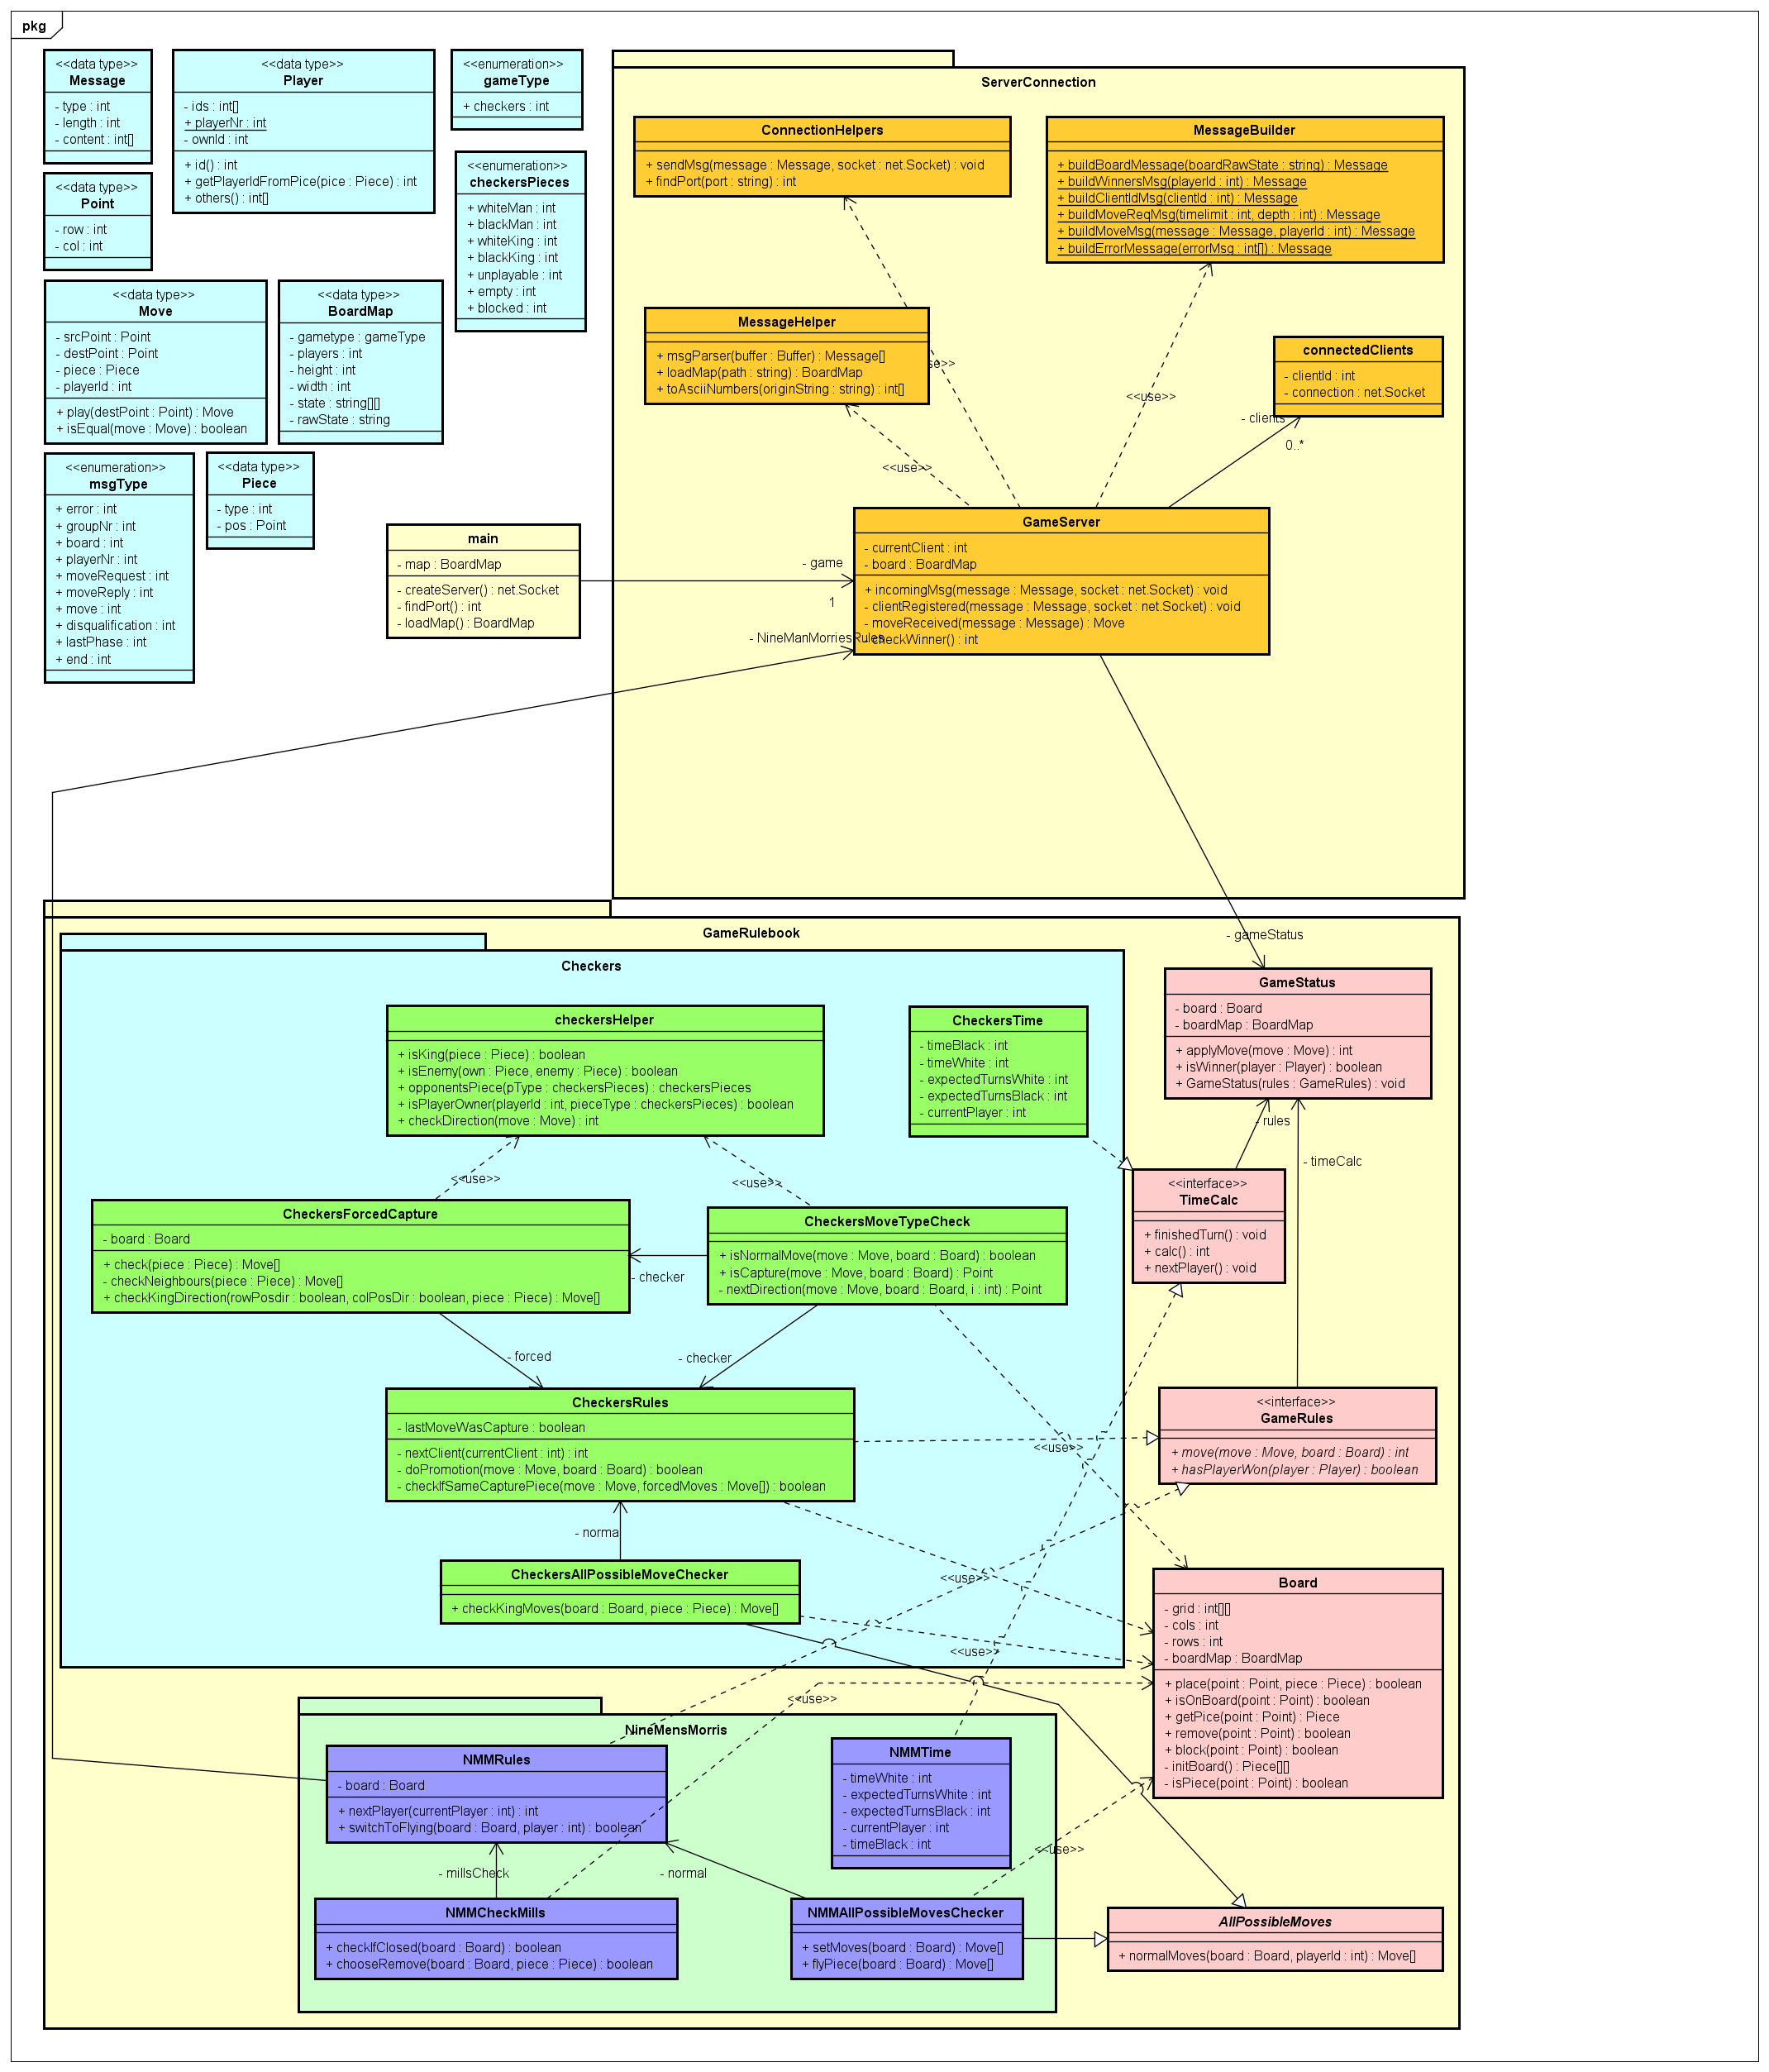
\includegraphics[width=1.0\linewidth]{pics/GameServerClassDiagram.png}
	\captionof{figure}[ClassDiagram]{ Das UML Klassendiagramm des Gameservers }
	\label{fig:GameServerClassDiagram}
\end{minipage}

\subsection{ReversiXT GUI}
Die ReversiXT Graphische Oberfläche (GUI) ist der Teil der Software der für die eigentliche Userinteraktion gedacht ist. User Können über die GUI
spiele starten, bei welchen sie gegen KI's oder andere User spielen können.

\subsubsection{Softwareaufbau der ReversiXT GUI}
Die ReversiXT GUI besteht aus zwei Teilen, dem Server und dem Webapp-Paket, siehe \ref{fig:ReversiXTGUIClassDiagram}. 
Dabei behandelt der Server, die Verbindung zu den anderen
Komponenten. Er startet den Gameserver und je nachdem wie viele KI's als Spieler gewählt werden, startet er auch die Gameclients dafür.
Sind die anderen Komponenten gestartet, kommunziert der Server der ReversiXT GUI nur noch mit Gameserver und benutzt dabei das Protokoll
welches dieser vorschreibt. Die Webapp behinhaltet das Benutzer Interface, über welches die Software für den Endnutzer bedient werden kann.
Über das Menü kann kann die Gameselection augerufen werden, bei welcher die verfügbaren Spiele ausgewählt werden können.
Wird ein Spiel ausgewählt, gibt es ein weiteres Menü über dass Spielspezifische Parameter einstellbar sind. 
Die Spiele sind als eigene Pakete eingegliedert und behinhalten, je nach Spiel ein Spielbrett und Möglichkeiten mittels Touch-Berührungen
Züge auszuführen. Durch diese Untergliederung in weitere Pakete kann die Software leicht um weitere Spiele erweitert werden.

\vspace{1em}
\begin{minipage}{\linewidth}
	\centering
	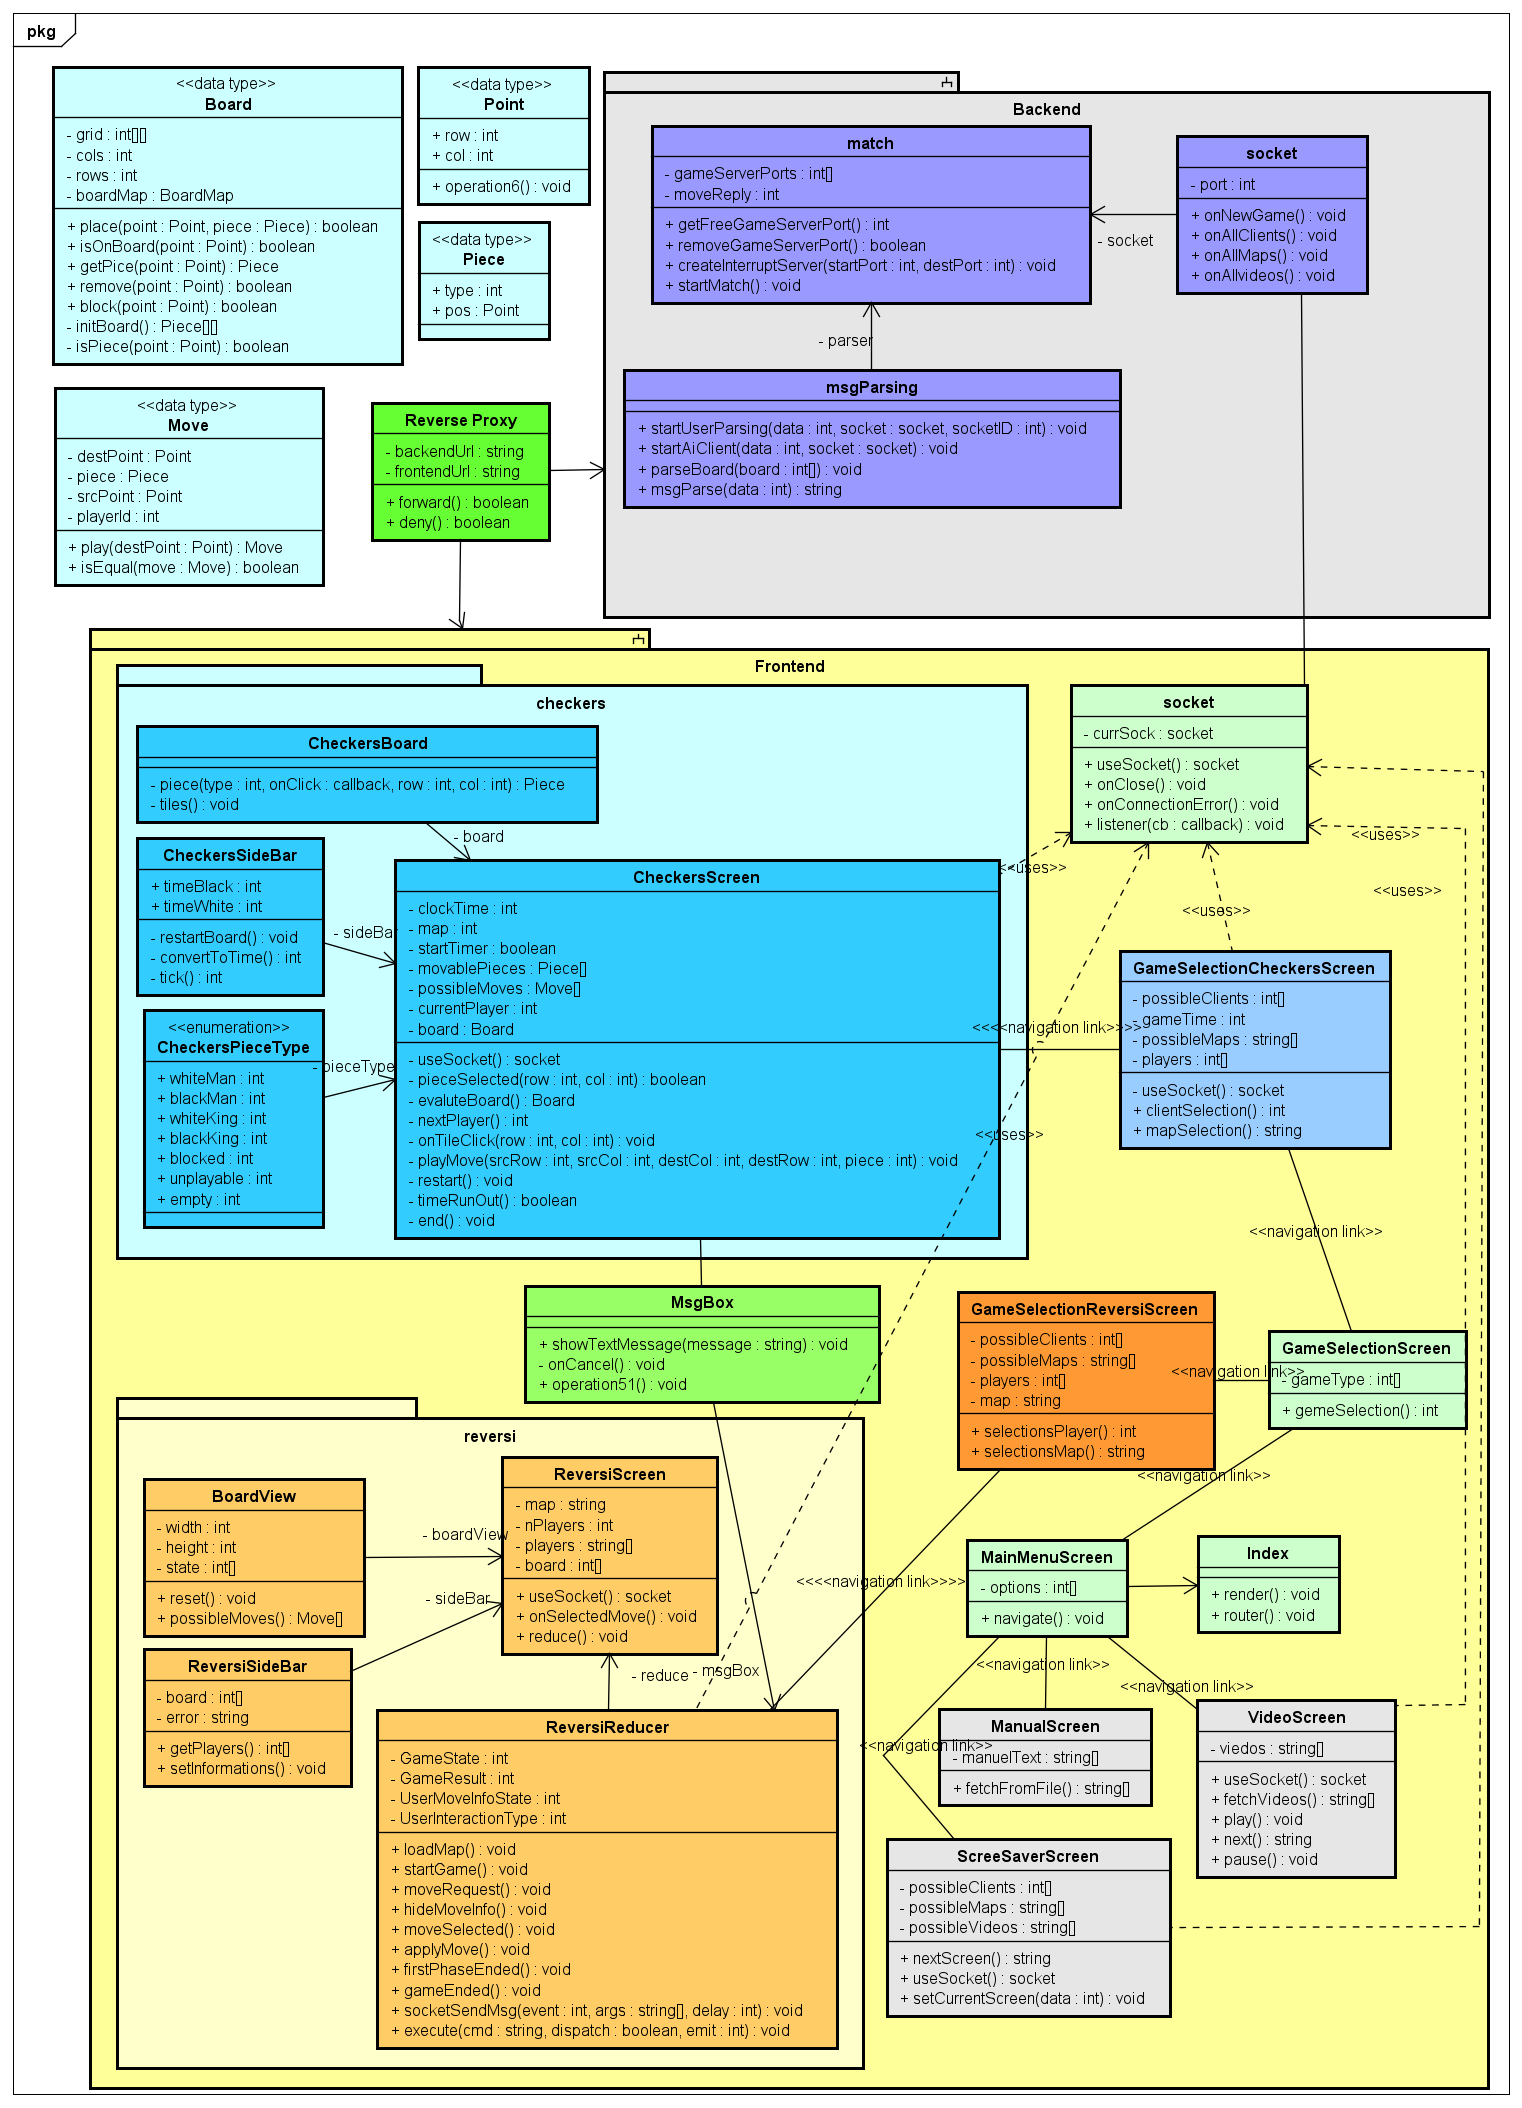
\includegraphics[width=0.9\linewidth]{pics/ReversiXTGUIClassDiagramm.png}
	\captionof{figure}[ReversiXTGUI]{ Das UML Klassendiagramm der ReversiXT GUI }
	\label{fig:ReversiXTGUIClassDiagram}
\end{minipage}




\subsection{KI Client}
Der KI Client beinhaltet die Logik der Künstlichen Intelligenz der Applikation. Wird ein Spiel gegen einen KI Client gestartet, so wird dieser gestartet und agiert als 
Gegenspieler zum User. Der User kann auch ein Spiel bei welchem zwei KI's gegeneinander spielen starten, wodurch zwei KI Clients gestartet werden.

\subsubsection{Softwareaufbau des KI Clients}
Der KI Client besteht aus drei Paketen, der KI-Logik, der Spielelogik und der Serververbindungslogik, siehe \ref{fig:KIClientClassDiagram}. 
Die Spielelogik, beeinhaltet ein Momentanzustand des Spielbrettes, sowie Möglichkeiten dieses nach belieben zu modifizieren. Das KI-Paket benutzt diese Logik um 
Züge auf auszuwerten und den bestmöglichen Zug zu wählen. Um verschiedene KI-Algorithmen verwenden zu können wird ein Interface bereit gestellt, wird die Applikation 
um einen weiteren KI-Algorithmus erweitert, so muss dieser das Interface verwenden. Wird eine Auswertung des Nächsten besten Zuges abeschlossen, so sendet das KI-Paket sein
Ergebnis an die das Server-Paket. Dieses ist verantwortlich für das Versenden und kodieren der Nachrichten. Nachrichten werden vom KI-Client zum Gameserver geschickt und müssen
dabei das Protokoll von diesem einhalten.

\vspace{1em}
\begin{minipage}{\linewidth}
	\centering
	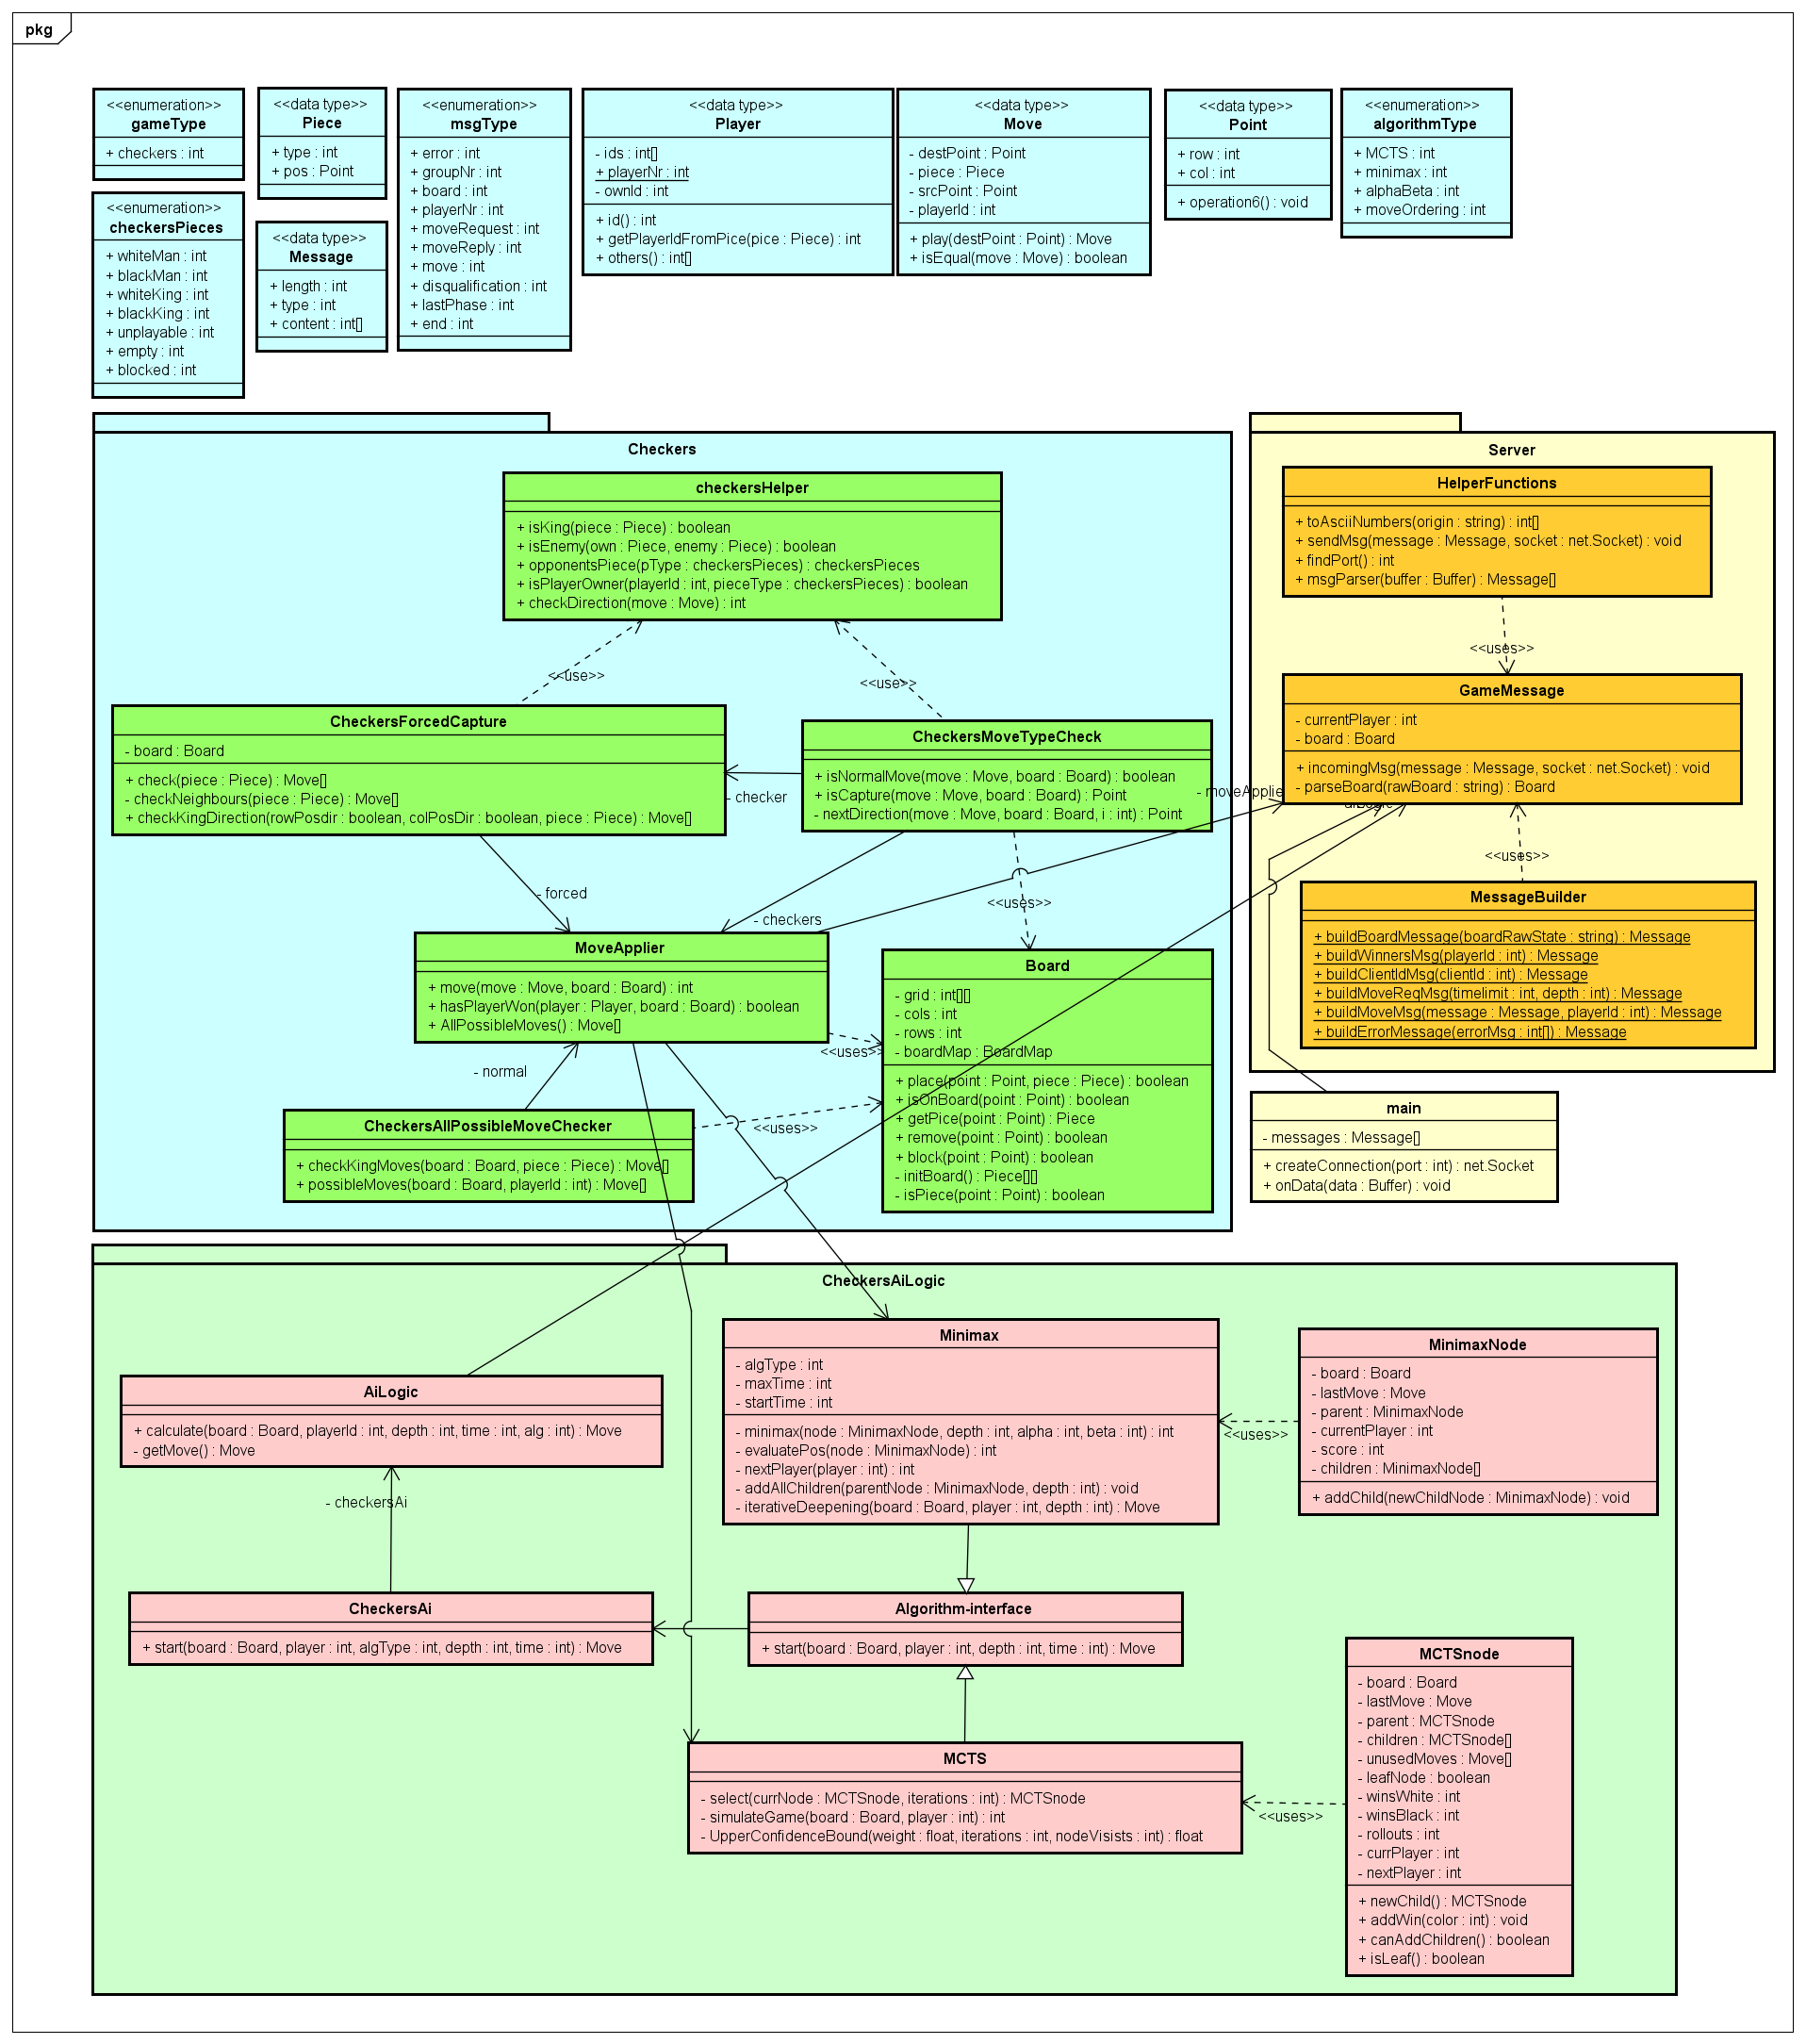
\includegraphics[width=0.9\linewidth]{pics/GameClientClassDiagram.png}
	\captionof{figure}[KIClient]{ Das UML Klassendiagramm des KI Clients }
	\label{fig:KIClientClassDiagram}
\end{minipage}


\section{Hardware}
Dieses Kapitel handelt von der verwendeten Hardware auf der die Software zum läuft. 
Die Software wird auf einem Raspberry Pi, welcher an einem Touch Monitor anschlossen ist ausgeführt.
\subsection{Raspberry Pi}
\subsection{Touch Monitor}

\section{Implementierung}
\subsection{Eingesetzte Sofwarekomponenten}
\subsubsection{Programmiersprachen und Frameworks}
\subsubsection{Datentransferprotokolle}
\subsection{Gameserver}
\subsubsection{Netzwerkspezifikation des Gameservers}
\subsection{Graphische Oberfläche}
\subsubsection{Gegebene React Anwendung}
\subsubsection{Erweiterungen}
\subsection{KI Client}
\subsubsection{Vergleich der KI Algorithmen}

\section{Testing}
\subsection{Integrationstest}
\subsection{Ergebnisse}

\pagebreak
% ----------------------------------------------------------------------------------
% Kapitel: Fazit und Ausblick
% ----------------------------------------------------------------------------------
\section{Fazit und Ausblick}



\pagebreak
% ----------------------------------------------------------------------------------
% Kleine Einführung in LaTeX-Elemente
% ----------------------------------------------------------------------------------
%\section{\LaTeX-Elemente}
%Dieser Abschnitt beinhaltet lediglich einige Informationen über \LaTeX-Distributionen, Editoren und \LaTeX-Elemente, die Ihnen beim Einstieg in das \LaTeX-Textsatzsystem helfen sollen.
%
%\subsection{\LaTeX-Distributionen nach Betriebssystemen}
%
%\subsubsection{\LaTeX-Distributionen}
%Folgende Haupt-\LaTeX-Distributionen stehen Ihnen zur Verfügung:
%\begin{itemize}
%  \item Windows:\quad \texttt{MiKTeX}\quad Webseite:\quad\url{http://www.miktex.org}
%  \item Linux/Unix:\quad \texttt{TeX Live}\quad Webseite:\quad\url{http://tug.org/texlive/}
%  \item Mac OS:\quad \texttt{MacTeX}\quad Webseite:\quad\url{http://www.tug.org/mactex/}
%\end{itemize}
%
%\subsubsection{\LaTeX-Editoren}
%Auf folgenden Webseiten können Sie einige hilfreiche \LaTeX-Editoren finden:
%\begin{itemize}
%  \item Windows/Linux/Mac OS: \url{http://www.xm1math.net/texmaker/}
%  \item Windiws: \url{http://www.texniccenter.org/}
%  \item Mac OS: \url{http://pages.uoregon.edu/koch/texshop/}
%\end{itemize}
%
%Falls bei den oben genannten Editoren kein passender vorhanden war, findet sich auf Wikipedia eine Zusammenstellung vieler weiterer \LaTeX-Editoren:\\[1em]
%\hspace*{3cm}\url{https://en.wikipedia.org/wiki/Comparison_of_TeX_editors}
%
%
%\subsection{Bilder}
%Zum Einfügen eines Bildes, siehe Abbildung \ref{fig:reversi01}, werden die \texttt{minipage}-Umgebung und der Befehl \texttt{$\backslash$includegraphics} genutzt, da die Bilder so gut positioniert und einfach integriert und skaliert werden können.
%
%\vspace{1em}
%\begin{minipage}{\linewidth}
%	\centering
%	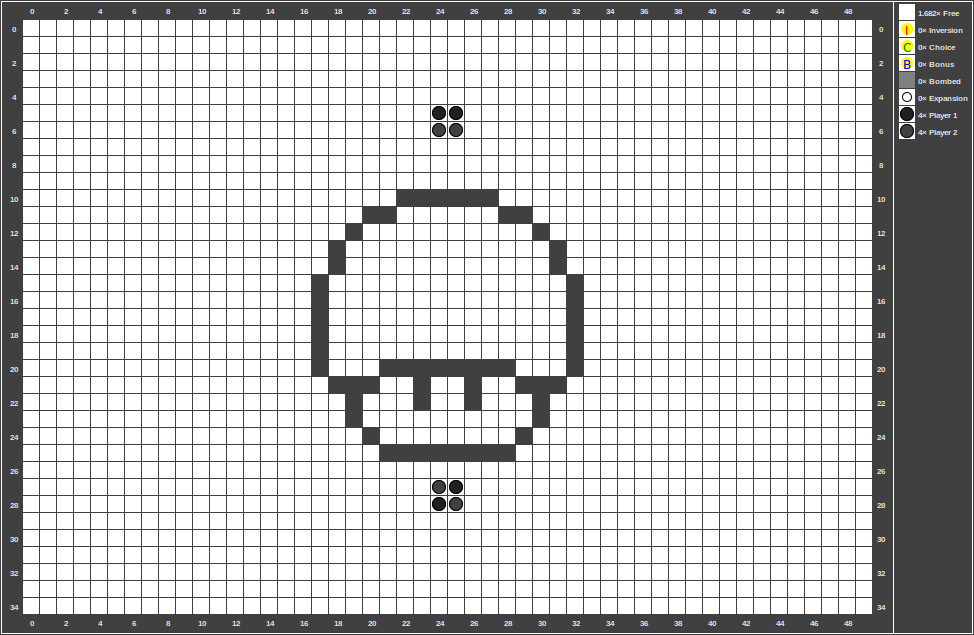
\includegraphics[width=0.5\linewidth]{pics/gamefield01.png}
%	\captionof{figure}[Spielfeld 01]{Unbespieltes Spielfeld\footnotemark }
%	\label{fig:reversi01}
%\end{minipage}
%\footnotetext{Diesem Spielfeld wurden noch keine Spieler zugewiesen (daher die dunklen Spielsteine)}
%
%Nachdem das Spielt gestartet wurde und beide Spielphasen durchlaufen wurden, siegt schließlich der Spieler mit der Farbe rot.
%
%\vspace{1em}
%\begin{minipage}{\linewidth}
%	\centering
%	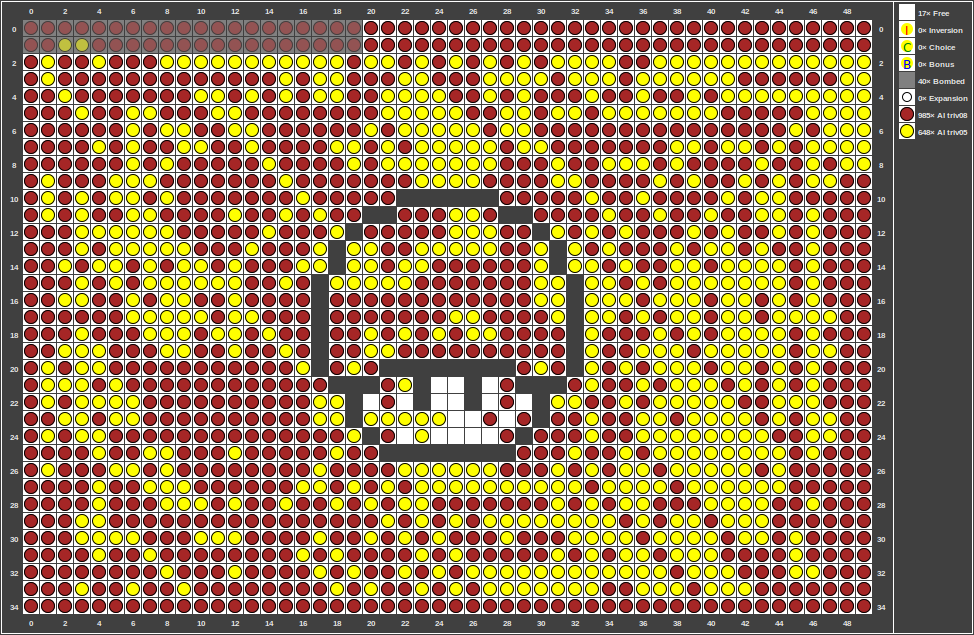
\includegraphics[width=0.5\linewidth]{pics/gamefield02.png}
%	\captionof{figure}[Spielfeld 02]{Finales Spielfeld\footnotemark }
%	\label{fig:reversi2}
%\end{minipage}
%\footnotetext{Das Spielfeld nach der Zug- und Bombenphase. Spieler rot gewinnt eindeutig.}
%
%\subsection{Tabellen}
%In diesem Abschnitt wird eine Tabelle (siehe Tabelle \ref{tab:beispiel}) dargestellt.
%
%\vspace{1em}
%\begin{table}[!h]
%	\centering
%	\begin{tabular}{|l|l|l|}
%		\hline
%		\textbf{Name} & \textbf{Name} & \textbf{Name}\\
%		\hline
%		1 & 2 & 3\\
%		\hline
%		4 & 5 & 6\\
%		\hline
%		7 & 8 & 9\\
%		\hline
%	\end{tabular}
%	\caption{Beispieltabelle}
%	\label{tab:beispiel}
%\end{table}
%
%
%\subsection{Auflistung}
%Für Auflistungen wird die \texttt{enumerate}- oder \texttt{itemize}-Umgebung genutzt.
%
%\begin{itemize}
%	\item Nur
%	\item ein
%	\item Beispiel.
%\end{itemize}
%
%\subsection{Listings}
%Zuletzt sehen Sie in Listing \ref{lst:maxTeilsumZweiD} ein Beispiel für das Einbinden von Quellcode mit Syntax-Highlighting.
%
%\vspace{1em}
%\lstinputlisting[caption=Brute Force-Ansatz für das MaxTeilsum2D-Problem, label=lst:maxTeilsumZweiD,basicstyle=\ttfamily\scriptsize]{code/maxTeilsum2DBruteForce.txt}
%
%\subsection{Selbstgestaltete Abbildungen}
%Mithilfe des Paketes \texttt{tikz} können sehr schöne Abbildungen (z.\,B.\ Automaten, Graphen etc.) direkt in \LaTeX generiert werden. Viele Beispiele dazu finden Sie auf folgender Webseite:\\[1em]
%\hspace*{3cm}\url{http://www.texample.net/tikz/}.
%
%\subsection{Tipps}
%Die Literaturreferenzen (Bücher, Paper und Journals) und Internetquellen (Webseiten, Blogs etc.) befinden sich in der Datei \textit{literatur.bib}. Eine Buch- und eine Online-Quelle sind beispielhaft eingefügt. [Vgl.\ \cite{buch}, \cite{mathcomm}]
%
%Literatur und Quellen werden in zwei getrennte Verzeichnisse aufgeteilt. Als Unterscheidungsmerkmal dient bei den Quellen der Zusatz: \texttt{keywords = \{online\}}.

\pagebreak

% ----------------------------------------------------------------------------------------------------------
% Filter fuer Literatur und Quellen definieren
% ----------------------------------------------------------------------------------------------------------

\defbibheading{Literatur}{\section*{Literaturverzeichnis}} 
\defbibheading{Quellen}{\section*{Quellenverzeichnis}} 
  
\defbibfilter{Literatur}{\not\keyword{online}} 
\defbibfilter{Quellen}{\keyword{online}} 


 ----------------------------------------------------------------------------------------------------------
 Literatur
 ----------------------------------------------------------------------------------------------------------
\lhead{} 
\rhead{Literaturverzeichnis} 

\printbibliography[heading=Literatur,filter=Literatur] 

\pagebreak


% ---------------------------------------------------------------------------------------------------------- 
% Quellen 
% ---------------------------------------------------------------------------------------------------------- 
\lhead{} 
\rhead{Quellenverzeichnis} 

\printbibliography[title = {Quellenverzeichnis}, heading=Quellen,filter=Quellen] 

\pagebreak 

% ----------------------------------------------------------------------------------------------------------
% Anhang
% ----------------------------------------------------------------------------------------------------------
\pagenumbering{Roman}
\setcounter{page}{1}
\lhead{Anhang \thesection}

\begin{appendix}
\section*{Anhang}
\phantomsection
\addcontentsline{toc}{section}{Anhang}
\addtocontents{toc}{\vspace{-0.5em}}

Inhalt des beigefügten Datenträgers:
\begin{itemize}
  \item $\ldots$
  \item $\ldots$
\end{itemize}

\section{Domändenmodell}
Ein toller Anhang, der nicht nur als \glqq{}\emph{Müllhalde}\grqq{} genutzt wird, sondern in dem Bilder und Inhalte auch mit eigenen Worten erklärt werden und den man auch für sich alleine lesen kann. Es sollten auch Referenzen auf die zugehörige ausführliche Behandlung im Hauptteil inklusive Seitenangabe mit $\backslash$\texttt{pageref} gegeben werden.

\subsection*{Screenshot}
\label{app:screenshot}
Unterkategorie, die nicht im Inhaltsverzeichnis auftaucht.

\end{appendix}


\pagebreak




\end{document}
